\documentclass[a4paper, 12pt]{article} % Artikel-Klasse

%---------------------------------------------------------
% Encoding, language, quotes
%---------------------------------------------------------
\usepackage[utf8]{inputenc}
\usepackage[ngerman]{babel}       % Deutsche Sprache und Silbentrennung
\usepackage{csquotes}             % Für korrekte Anführungszeichen
\usepackage{listings}
\usepackage{xcolor}

%---------------------------------------------------------
% Graphics & PDF
%---------------------------------------------------------
\usepackage{graphicx}
\usepackage{pdfpages}             % Einbinden von PDF-Seiten
\usepackage{caption}              % Verbesserte Bildunterschriften
\usepackage{subcaption}

% Customize settings
% Customize settings for a more compact style
\lstset{
    language=Java,                 % Specify Java language for syntax highlighting
    basicstyle=\ttfamily\small,    % Use smaller monospaced font for code
    keywordstyle=\color{blue},     % Style for keywords
    commentstyle=\color{gray},     % Style for comments
    stringstyle=\color{red},       % Style for strings
    numbers=none,                  % No line numbers
    breaklines=true,               % Break long lines
    frame=none,                    % No frame around the code
    xleftmargin=0pt,               % Remove left margin
    xrightmargin=0pt,              % Remove right margin
    aboveskip=5pt,                 % Reduce space above the code block
    belowskip=5pt                  % Reduce space below the code block
}

%---------------------------------------------------------
% Math, units, spacing, etc.
%---------------------------------------------------------
\usepackage{siunitx}
\usepackage{setspace}
\usepackage{textgreek}

% Add float package for "H" float option
\usepackage{float}

%---------------------------------------------------------
% Other packages
%---------------------------------------------------------
\usepackage{ifthen}
\usepackage{acronym}
\PassOptionsToPackage{hyphens}{url} % URLs in Hyperlinks umbrechen
\usepackage[breaklinks=true]{hyperref} 
\usepackage{array}                % Bessere Tabellenformatierung
\usepackage{enumitem}             % Kontrolle über Listen-Layouts
\usepackage{nomencl}
\usepackage{scrlayer-scrpage}     % Header und Footer

% Adjust header and footer heights
\setlength{\headheight}{14.5pt}
\setlength{\footheight}{34.16666pt}

%---------------------------------------------------------
% Bibliography (biblatex mit Biber)
%---------------------------------------------------------
\usepackage[backend=biber, style=ieee]{biblatex}  
\addbibresource{literatur.bib}  

%---------------------------------------------------------
% Platzhalter
%---------------------------------------------------------
\newcommand{\titel}{Entwicklung eines mobilen Warnsystems zur Minimierung von Abbiegeunfällen zwischen LKW und Fußgänger*innen}
\newcommand{\untertitel}{}
\newcommand{\arbeit}{Studienarbeit T3100}
\newcommand{\studiengang}{Elektrotechnik}
\newcommand{\studienrichtung}{Fahrzeugelektronik}
\newcommand{\autor}{Luka Tadic}
\newcommand{\abgabe}{13.01.2025}
\newcommand{\bearbeitungszeitraum}{09.10.2024 - 13.01.2025}
\newcommand{\matrikelnr}{5726700}
\newcommand{\kurs}{TFE22-1}
\newcommand{\firma}{}
\newcommand{\betreuerfirma}{Prof. Dr. Ing. Tobias Frank}
\newcommand{\gutachterdhbw}{Prof. Dr. Ing. Tobias Frank}
\newcommand{\jahr}{2025}

%---------------------------------------------------------
% Header und Footer mit Linien
%---------------------------------------------------------
\clearpairofpagestyles         % Standard-Stile löschen

% Header with consistent logo placement and line position
\ohead{%
    \raisebox{1cm}[0pt][0pt]{% Raise the logo well above the line
        
\includegraphics[width=3cm]{images/DHBW_d_R_FN_46mm_4c}%
    }%
    \\[-1.5cm] % Move the header line down
    \rule{\textwidth}{0.4pt} % Horizontal rule for the header line
}


% Footer with consistent alignment and contents below the line
\setkomafont{pagefoot}{\normalfont} % Ensure consistent font style
\cfoot{%
    \rule{\textwidth}{0.4pt}\\ % Horizontal rule
    \vspace{0.3em} % Small vertical space
    \begin{tabular}{@{}p{0.33\textwidth}p{0.33\textwidth}p{0.33\textwidth}@{}}
        \arbeit & \centering \autor & \raggedleft \thepage
    \end{tabular}
}


\pagestyle{scrheadings}        % Stil aktivieren

%---------------------------------------------------------
% Dokumentbeginn
%---------------------------------------------------------
\begin{document}
\sloppy

%---------------------------------------------------------
% Titelseite
%---------------------------------------------------------
\thispagestyle{empty}  % Kein Header oder Footer auf der Titelseite
\hypersetup{pageanchor=false}

\begin{titlepage}
\enlargethispage{4.0cm}
\sffamily  % Serifenlose Schrift für die Titelseite

\parbox{0.5\linewidth}{
    \begin{flushleft}
        % Optional: Firmenlogo
    \end{flushleft}
}
\parbox{0.5\linewidth}{
    \begin{flushright}
        
\includegraphics[width=0.4\linewidth]{images/DHBW_d_R_FN_46mm_4c}\\[5ex]
    \end{flushright}
}

\begin{center}

{\fontsize{20.74pt}{24pt}\selectfont
\textbf{\titel}\\[1.5ex]}

{\fontsize{17pt}{20pt}\selectfont
\textbf{\arbeit}\\[2ex]}

{\fontsize{14pt}{17pt}\selectfont
Studiengang \studiengang\\[2ex]}

{\fontsize{12pt}{14pt}\selectfont
Studienrichtung \studienrichtung\\[1ex]
Duale Hochschule Baden-Württemberg Ravensburg, Campus Friedrichshafen\\[5ex]
von\\[1ex]
\autor\\[15ex]}

\end{center}

\begin{center}
{\fontsize{12pt}{14pt}\selectfont
\begin{tabular}{ll}
Abgabedatum:                    & \quad \abgabe \\  
Bearbeitungszeitraum:           & \quad \bearbeitungszeitraum \\  
Matrikelnummer:                 & \quad \matrikelnr \\  
Kurs:                           & \quad \kurs \\  
Dualer Partner:                 & \quad \firma \\ % entfällt bei Studienarbeit
Betreuerin / Betreuer:          & \quad \betreuerfirma \\  
Gutachterin / Gutachter:        & \quad \gutachterdhbw \\ [2ex]
\end{tabular}
}
\end{center}

\end{titlepage}

\clearpage

\pagestyle{scrheadings}  % Header und Footer nach Titelseite aktivieren
\hypersetup{pageanchor=true}

%---------------------------------------------------------
% Erklärung
%---------------------------------------------------------

\pagenumbering{Roman}

\section*{Erklärung}

Ich versichere hiermit, dass ich meine \arbeit\ mit dem Thema:

\begin{quote}
    \textit{\titel}
\end{quote}

selbstständig verfasst und keine anderen als die angegebenen Quellen und Hilfsmittel benutzt habe.  
Ich versichere zudem, dass die eingereichte elektronische Fassung mit der gedruckten Fassung übereinstimmt.\\[6ex]

Friedrichshafen, den \today \\[1ex]
\rule[-0.2cm]{5cm}{0.5pt} \\  
\autor \\[10ex]

\rmfamily

\clearpage

\section*{Kurzfassung}
\begin{spacing}{1.8}  % Adjust line spacing
    \fontsize{14pt}{14pt}\selectfont  % Font size and line spacing
    Die vorliegende Studienarbeit untersucht die Entwicklung eines mobilen Warnsystems zur Minimierung von Abbiegeunfällen zwischen LKW und ungeschützten Verkehrsteilnehmenden. Aufbauend auf früheren Forschungsarbeiten wurde ein Konzept entwickelt, das die
    Bluetooth-Angle-of-Arrival-Technologie (AoA) nutzt, um die Position 
    von Fußgängerinnen und Radfahrerinnen präzise zu bestimmen. Ziel ist
     die Entwicklung einer mobilen Applikation, die als Signalquelle für
      ein LKW-Abbiegeassistenzsystem dient. Diese App bietet eine 
      kostengünstige und zugängliche Lösung, um kritische 
      Verkehrssituationen frühzeitig zu erkennen und Warnungen auszugeben.

    Die Arbeit umfasst die Analyse der technischen Grundlagen 
    von Bluetooth, die Implementierung einer Android-App 
    für das Scannen 
    und Erkennen von Bluetooth-Geräten sowie die Konzeption 
    einer bidirektionalen Kommunikation zwischen App und LKW-System.
     Aktuelle Herausforderungen bestehen in der fehlenden 
     Senderfunktionalität der App und der unklaren Kompatibilität 
     mit der verwendeten Hardware.
    
    Zukünftige Arbeiten sollten die vollständige bidirektionale 
    Kommunikation, eine verbesserte Benutzerfreundlichkeit und
    plattformübergreifende Anwendungen fokussieren. Langfristig kann das System dazu beitragen, die Verkehrssicherheit signifikant zu erhöhen und Leben zu retten.

\end{spacing}
%---------------------------------------------------------
% Abstract
%---------------------------------------------------------
\section*{Abstract}
\begin{spacing}{1.8}  % Adjust line spacing
    \fontsize{14pt}{14pt}\selectfont  % Font size and line spacing
    This study examines the development of a mobile warning system to reduce turning accidents between trucks and vulnerable road users. Building on previous research, a concept was developed utilizing Bluetooth Angle-of-Arrival (AoA) technology 
    to precisely determine the position of pedestrians and cyclists.
    The goal is to create a mobile application that acts as a signal 
    emitter for a truck turn-assistance system, providing an affordable
     and accessible solution for early detection of critical traffic 
     situations and issuing warnings.

    The work includes an analysis of the technical 
    foundations of Bluetooth, the implementation of an Android 
    app for scanning and detecting Bluetooth devices, 
    and the conceptualization of bidirectional communication
     between the app and the truck system. Current challenges 
     include the lack of signal-emitting functionality in the app 
     and unclear compatibility with the chosen hardware.
    
    Future developments should prioritize achieving complete 
    bidirectional communication, enhancing user-friendliness, 
    and extending the solution to other platforms. In the long term,
     the system has the potential to significantly improve traffic safety
      and save lives.

\end{spacing}
\clearpage

\section*{Hilfsmittel}
\begin{spacing}{1.8}  % Adjust line spacing
    \fontsize{14pt}{15pt}\selectfont  % Font size and line spacing

    Im Rahmen dieser Arbeit wurden verschiedene Hilfsmittel verwendet, von denen
    insbesondere der Einsatz von LLMs (Large Language Models) von Bedeutung ist.
    
    Die Autoren haben LLMs, wie beispielsweise ChatGPT, genutzt, um allgemeinen
    Code (z.B. Klassen und Funktionskörper) für die Arbeit implementieren zu lassen.
    Es ist den Autoren wichtig zu betonen, dass die dem Projekt zugrunde liegende
    Algorithmik, sofern nicht anders gekennzeichnet, selbst entwickelt wurde und auf
    eigenem Gedankengut basiert.

\end{spacing}

\clearpage
% List of figures
\addcontentsline*{toc}{section}{}  % Add section to table of contents
\listoffigures

\clearpage

\section*{Abkürzungsverzeichnis}
\begin{spacing}{1.8}  % Adjust line spacing
    \fontsize{14pt}{15pt}\selectfont  % Font size and line spacing

   \textbf{AoA}  - Angle-of-Arrival

   \textbf{API} - Application Programming Interface

   \textbf{BLE} - Bluetooth Low Energy

   \textbf{DHBW} - Duale Hochschule Baden-Württemberg

   \textbf{FHSS} - Frequency Hopping Spread Spectrum

   \textbf{ISM} - Industrial, Scientific, Medical

   \textbf{LKW} - Lastkraftwagen

   \textbf{DSGVO} - Datenschutz-Grundverordnung

   \textbf{UI} - User Interface

   \textbf{UX} - User Experience

   \textbf(XML) - Extensible Markup Language


\end{spacing}

\clearpage


%---------------------------------------------------------
% Inhaltsverzeichnis
%---------------------------------------------------------
\tableofcontents

\clearpage

%---------------------------------------------------------
% Hauptkapitel
%---------------------------------------------------------
\pagenumbering{arabic}
\setcounter{page}{1}

\section{Einleitung}
\begin{spacing}{1.8}  % Adjust line spacing
    \fontsize{14pt}{15pt}\selectfont  % Font size and line spacing

\end{spacing}

    \subsection{Motivation}
\begin{spacing}{1.8}  % Adjust line spacing
    \fontsize{14pt}{15pt}\selectfont  % Font size and line spacing

    In den letzten Jahren ist die Zahl der tödlichen Verkehrsunfälle bedauerlicherweise
     gestiegen, was auf eine Vielzahl von Faktoren wie steigende
      Verkehrsdichte sowie mangelnde Aufmerksamkeit und Sorgfalt
       im Straßenverkehr zurückzuführen sein kann. Um dieser
        negativen Entwicklung entgegenzuwirken,
         wurden unterschiedliche Maßnahmen ergriffen. 
         Neben strengeren Sicherheitsgesetzen haben sich vor 
         allem technologische Innovationen wie Fahrzeugkameras, Sensorik und verschiedene Fahrerassistenzsysteme als wesentliche
          Instrumente zur Unfallprävention herauskristallisiert.

        

Eine besonders bedeutende Neuerung im Bereich 
der LKW-Sicherheit stellen Abbiegeassistenten dar.
 Diese Systeme helfen, den toten Winkel zu reduzieren und somit
  Unfälle – insbesondere beim Rechtsabbiegen – zu vermeiden. Trotz dieser technischen Fortschritte besteht 
  weiterhin Potenzial für weitere Verbesserungen. Eine umfassende Forschung und Entwicklung im Bereich von Fahrerassistenzsystemen könnte zukünftig dazu beitragen, 
  das allgemeine Verkehrsrisiko weiter zu senken und die Verkehrssicherheit signifikant zu erhöhen \cite{grunder_simon_2024}.
\end{spacing}

\clearpage

\subsection{Zielsetzung}
\begin{spacing}{1.8}  % Adjust line spacing
    \fontsize{14pt}{15pt}\selectfont

    Die vorliegende Studienarbeit baut auf den Ergebnissen von C.
     Gründer und J. Simon\cite{grunder_simon_2024} sowie von A. D. Gardy\cite{gardy_andy_2023} auf.
      In der Arbeit von Gründer und Simon wurde ein Prototyp für ein LKW-Abbiegeassistenzsystem entwickelt, das die Position von Fahrradfahrenden mithilfe von Bluetooth erfasst. Gardy wiederum realisierte 
      eine winkelbasierte Bluetooth-Ortung über einen intelligenten Fahrradhelm, der als 
      Signal-Emitter fungierte. Dadurch können kritische Situationen beim Abbiegen erkannt und 
      frühzeitig Warnungen ausgegeben werden.

Ziel dieser Arbeit ist es, das in \cite{grunder_simon_2024} und \cite{gardy_andy_2023} skizzierte Konzept der Bluetooth-basierten 
Positionsbestimmung auf eine breitere Anwendungsebene zu heben. Statt wie bisher die 
Funktionalität auf einen speziellen Fahrradhelm zu beschränken, soll eine mobile Applikation 
entwickelt werden, die für sämtliche Verkehrsteilnehmende zugänglich ist. Diese App übernimmt
 die Rolle des Signal-Emitters und ermöglicht somit eine weitaus flexiblere und 
 kostengünstigere Implementierung. Durch die Einbindung in gängige mobile Endgeräte soll sich 
 die Technologie auch für
 Fußgänger*innen oder Personen, die kein spezielles Helmsystem 
 verwenden, eignen.

Darüber hinaus sollen Optimierungen in den Bereichen Datenverarbeitung 
und -auswertung vorgenommen werden, um eine noch präzisere 
Positionsbestimmung zu erreichen und Fehlalarme zu reduzieren. 
Hierbei wird weiterhin auf die vorhandene Hardware-Infrastruktur, 
wie das XPLR-AOA Explorer Kit von u-blox, zurückgegriffen, allerdings 
mit dem Fokus auf eine verbesserte Software-Architektur und benutzerfreundliche 
Anwendungsentwicklung. 

\begin{figure}[H]
    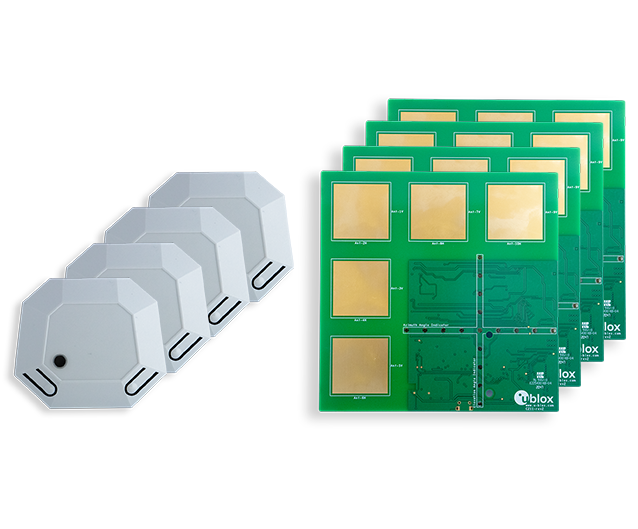
\includegraphics[width=0.8\linewidth]{images/XPLR-AOA-with-C209-and-C211-02_0}\\[1ex]
    \centering
    \caption{XPLR-AOA Explorer Kit \cite{u_blox_xplr_aoa2_kit}}
    \label{ABBILDUNG 76}
\end{figure}

Das übergeordnete Ziel ist es, die Verkehrssicherheit insbesondere beim 
Abbiegen von LKW signifikant zu erhöhen und dadurch Unfallzahlen zu reduzieren.

\end{spacing}

\clearpage

\section{Idee und Konzept}
\label{sec:Idee und Konzept}




\begin{spacing}{1.8}  % Adjust line spacing
\fontsize{14pt}{15pt}\selectfont  % Font size and line spacing

 
Im vorliegenden Projekt soll eine mobile Anwendung entwickelt werden, die sowohl als Empfänger als auch als Sender von relevanten Positions- und Warninformationen agieren kann. Anders als in bisherigen Ansätzen, bei denen die Funktionsweise größtenteils auf wenige Verkehrsteilnehmende (z. B. Personen mit speziellen Helmen) beschränkt war, soll mit dieser App eine breite Nutzerbasis angesprochen werden.  

Ziel ist es, dass sowohl LKW-Fahrende als auch Fußgänger*innen beziehungsweise weitere ungeschützte Verkehrsteilnehmende gleichermaßen von dem System profitieren. Konkret werden folgende Hauptfunktionen angestrebt:

1. Senderfunktion: 
   Die App auf dem Smartphone eines Fußgängers oder einer Fußgängerin fungiert als Signalquelle. Die vom mobilen Endgerät ausgesendeten Bluetooth-Signale ermöglichen es einem im LKW befindlichen Assistenzsystem, die relative Position zu erfassen und eine Warnung an den oder die LKW-Fahrende auszugeben, sobald eine kritische Abbiegesituation erkannt wird.

2. Empfängerfunktion:  
   Umgekehrt kann die App eingehende Warnsignale des LKW-Abbiegesystems verarbeiten, sobald eine kritische Situation vorliegt. Als Reaktion darauf erfolgt beispielsweise eine Warnung via Vibration oder eine Bildschirmbenachrichtigung auf dem Smartphone des oder der Fußgänger\*in. Dadurch soll eine gegenseitige Wahrnehmung der Verkehrsteilnehmenden erreicht werden, um das Unfallrisiko weiter zu reduzieren.

Die Realisierung dieser bidirektionalen Kommunikation erfordert eine durchdachte Systemarchitektur, welche die folgenden Aspekte berücksichtigt:

\textbf{Datensicherheit und Datenschutz:}  Da personenbezogene Daten (z. B. Standortinformationen) erhoben werden, muss sichergestellt sein, dass sämtliche Prozesse DSGVO-konform gestaltet sind.  

\textbf{Robuste Bluetooth-Kommunikation:}  Die App muss in unterschiedlichsten Umgebungen, wie dicht besiedelten Stadtgebieten mit hohem Interferenzpotenzial, zuverlässig funktionieren.  

\textbf{Benutzerfreundlichkeit:}  Eine intuitive Bedienung und eine minimalinvasive Warnung (etwa durch eine kurze Vibration) erhöhen die Akzeptanz des Systems bei allen Verkehrsbeteiligten.  

\textbf{Skalierbarkeit:}  Sowohl technische Komponenten (z. B. Netzwerk- und Sensorlast) als auch die Benutzeranzahl sollten skalierbar sein, um eine möglichst breite Anwendung zu ermöglichen.

Durch die Kombination dieser Maßnahmen wird eine umfassende Lösung angestrebt, die auf den Erkenntnissen der Vorarbeiten aufbaut und die Verkehrssicherheit durch eine umfassende und zugängliche Warninfrastruktur verbessert.

\begin{figure}[H]
    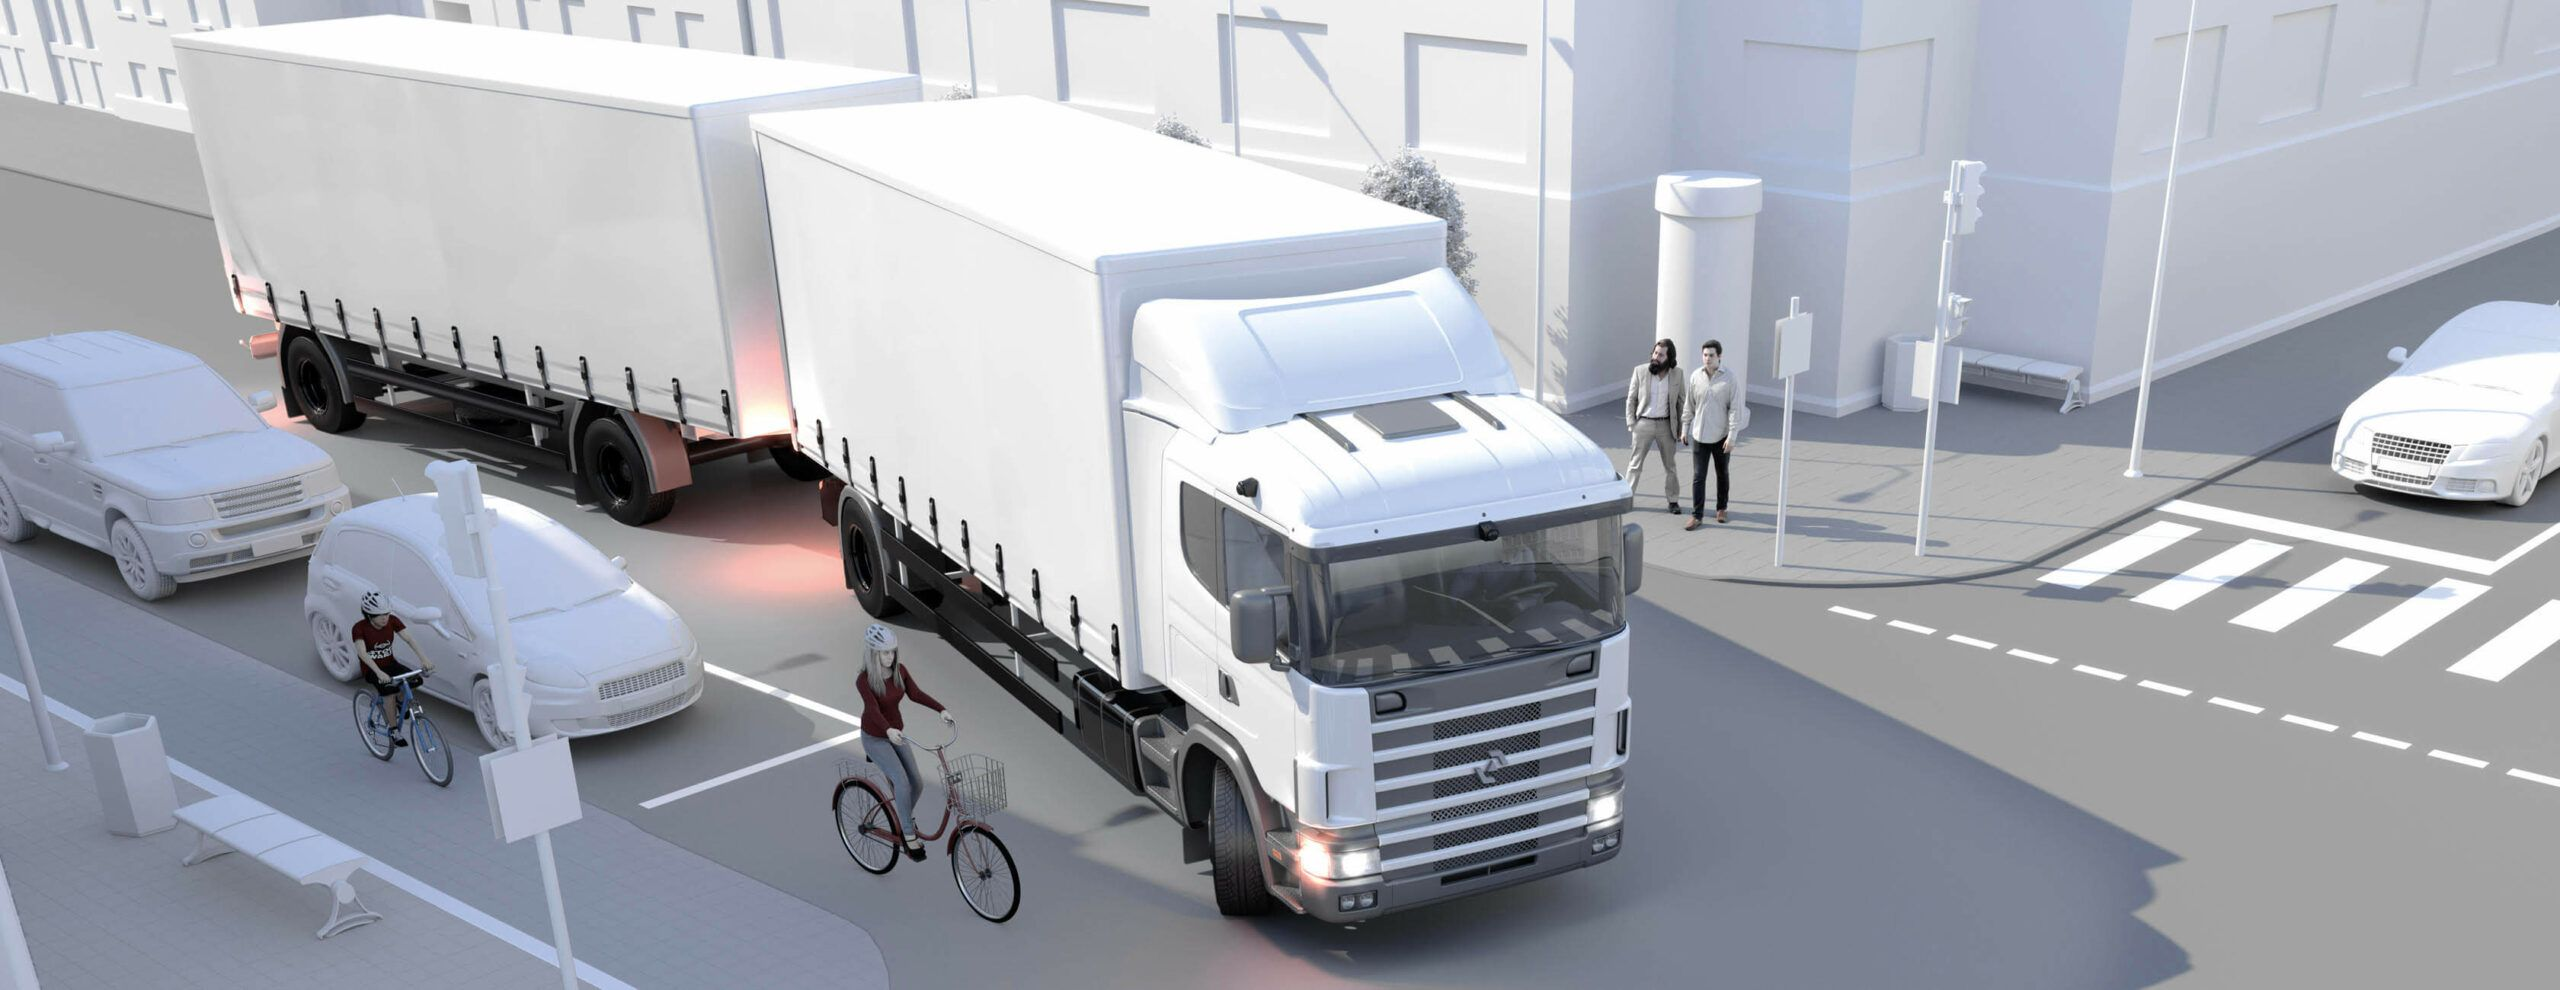
\includegraphics[width=1\linewidth]{images/abbiegeassistent-scaled-7b2478b8.jpeg}\\[1ex]
    \centering
    \caption{Beispiel LKW-Abbiegeassistenzsystem potentielle Situation\cite{abbiegeassistent_website}}
    \label{ABBILDUNG 76}
\end{figure}

\end{spacing}

\clearpage

\section{Anforderungen und Zielgruppe}


\begin{spacing}{1.8}  % Adjust line spacing
\fontsize{14pt}{15pt}\selectfont  % Font size and line spacing


Bei der Konzeption und Realisierung der mobilen Anwendung ist
 zu berücksichtigen, dass die zugrunde liegende Hardware auf dem 
 Bluetooth-Standard 5.1 basiert. Diese Version bringt insbesondere mit der 
 Angle-of-Arrival-(AoA)-Technologie einen wesentlichen Fortschritt in der Positionsbestimmung, da sie eine präzisere und schnellere Lokalisierung ermöglicht. Folglich ist für eine volle Funktionalität erforderlich, dass Endgeräte mindestens Bluetooth 5.1 oder höher unterstützen. 

Aufgrund der noch relativ geringen Verbreitung aktueller
 Bluetooth-Versionen kann dies zu einer eingeschränkten Nutzbarkeit führen. 
 Ein bedeutsamer Teil der zu entwickelnden Lösung besteht daher darin, durch 
 geeignete Design- und Implementierungsentscheidungen sowie durch klare Kommunikation gegenüber den Nutzenden sicherzustellen, dass das System trotz dieser technischen Voraussetzungen ein möglichst breites Anwendungsspektrum abdeckt.  


Da das System generell der Erhöhung der Verkehrssicherheit
 dienen soll, richtet es sich an alle Verkehrsteilnehmenden. Ein besonderer 
 Fokus liegt auf ungeschützten Personengruppen wie Fußgänger*innen und insbesondere Kindern. Da Letztere im Straßenverkehr ein erhöhtes Risiko aufweisen, ist eine intuitive und leicht verständliche Gestaltung der App von entscheidender Bedeutung.  

Darüber hinaus wird angestrebt, die App so zu
 gestalten, dass sie auch für ältere Personen oder Nutzer*innen mit wenig
  technischer Erfahrung einfach zu bedienen ist. Eine klare, barrierearme
   Benutzeroberfläche und ein einheitliches Warnkonzept sollen hier maßgeblich
    zur Nutzerakzeptanz und damit zum Erfolg der Anwendung beitragen.
\end{spacing}

\clearpage

\section{Bluetooth}

\begin{spacing}{1.8}  % Adjust line spacing
\fontsize{14pt}{15pt}\selectfont  % Font size and line spacing

Nachfolgend werden die für diese Arbeit relevanten Aspekte der Bluetooth-Technologie in einzelnen Unterkapiteln dargestellt.
 Dabei wird ein grundlegendes Verständnis für die Eigenschaften und Funktionsweisen von Bluetooth vermittelt, das als Fundament für das hier vorgestellte
 Abbiegeassistenzsystem dient.

\end{spacing}

\subsection{Allgemeine Grundlagen}

\begin{spacing}{1.8}  % Adjust line spacing
\fontsize{14pt}{15pt}\selectfont  % Font size and line spacing

Bluetooth ist ein Funkstandard, der im lizenzfreien 2,4-GHz-ISM-Band (Industrial, Scientific, Medical) betrieben wird und in erster Linie zur drahtlosen Kommunikation über kurze Entfernungen entwickelt wurde. Die Reichweite beträgt dabei üblicherweise etwa zehn Meter, kann jedoch – abhängig von der Hardwareklasse – zwischen einem und bis zu hundert Metern variieren. Aufgrund seiner einfachen Handhabung und vergleichsweise geringen Energieanforderungen findet Bluetooth in 
zahlreichen Alltagsgeräten wie Smartphones, Kopfhörern und Freisprecheinrichtungen Anwendung.

\end{spacing}

\subsection{Funktionsweise}

\begin{spacing}{1.8}  % Adjust line spacing
\fontsize{14pt}{15pt}\selectfont  % Font size and line spacing
Ein zentrales Element der Bluetooth-Kommunikation stellt das Frequenzsprungverfahren (Frequency Hopping Spread Spectrum, FHSS) dar, bei dem das System bis zu 1600 Mal pro Sekunde zwischen 79 (in einigen Regionen 40) Kanälen wechselt.
 Dieser Mechanismus dient insbesondere der Minimierung von Interferenzen mit anderen Funkdiensten, die ebenfalls das 2,4-GHz-Band nutzen (z. B. WLAN).

 \begin{figure}[H]
    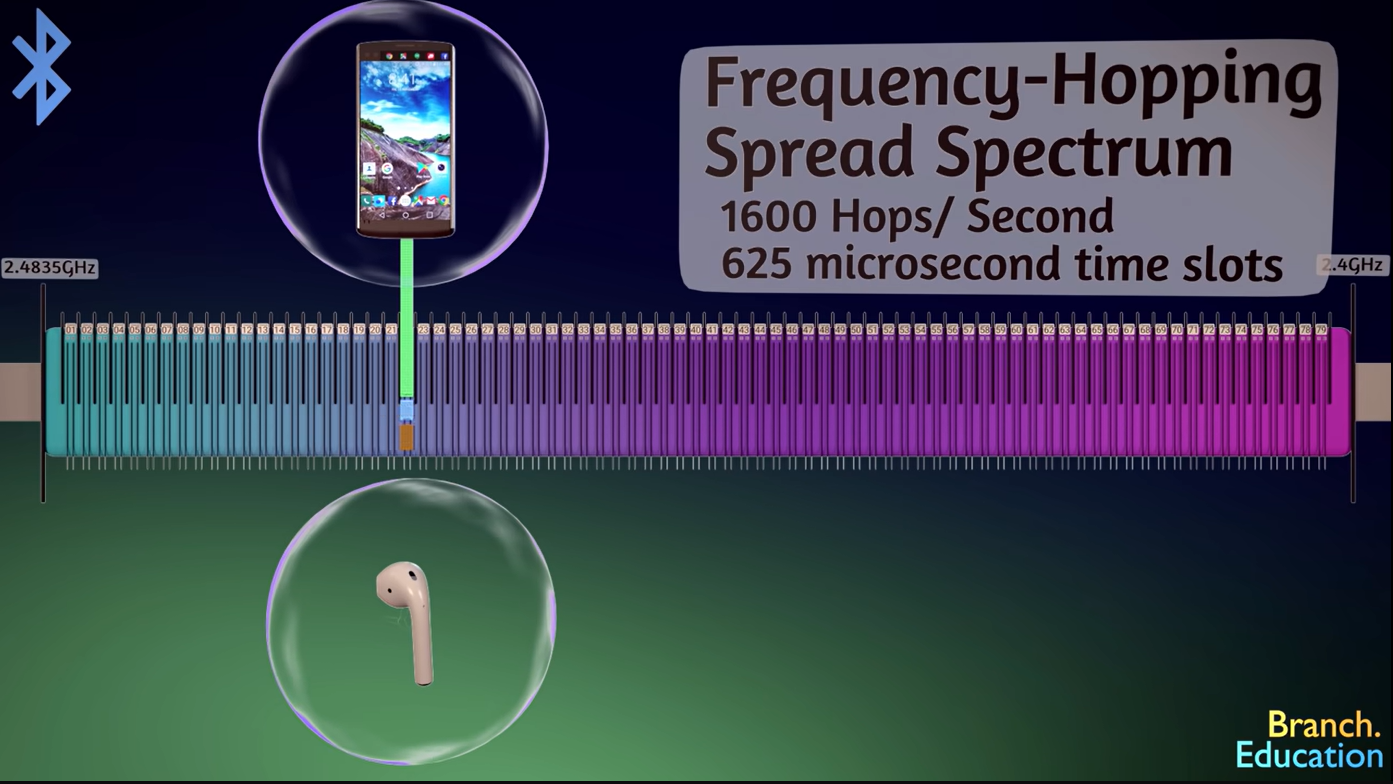
\includegraphics[width=1\linewidth]{images/2025-01-13_15h05_23.png}\\[1ex]
    \centering
    \caption{Modelldarstellung Bluetooth Datenübertragung(Frequency Hopping Spread Spectrum (FHSS)) \cite{branch_education_lidar_2023}}
    \label{ABBILDUNG 76}
\end{figure}

Bluetooth-Geräte werden zu sogenannten Piconets zusammengeschlossen.
 Innerhalb eines Piconets übernimmt ein Master-Gerät (z. B. ein Smartphone) die Verbindungssteuerung und verwaltet mehrere Slaves (z. B. drahtlose Kopfhörer). 
 Ein Master kann bis zu sieben aktive Slaves parallel betreiben, während weitere Geräte in einem passiven Modus verbleiben können.

 \begin{figure}[H]
    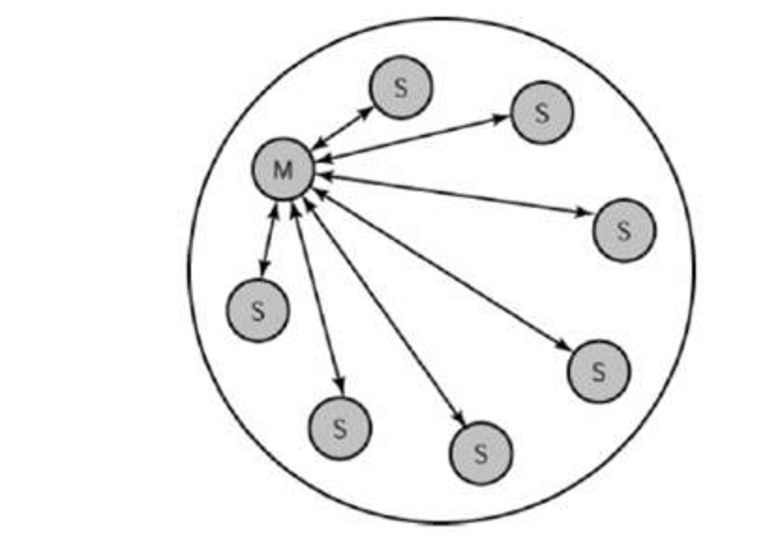
\includegraphics[width=1\linewidth]{images/Piconet.png}\\[1ex]
    \centering
    \caption{Piconets \cite{wikipedia_piconet}}
    \label{ABBILDUNG 76}
\end{figure}

\end{spacing}

\subsection{Verbindungsaufbau}

\begin{spacing}{1.8}  % Adjust line spacing
\fontsize{14pt}{15pt}\selectfont  % Font size and line spacing

Der Verbindungsaufbau zwischen zwei Bluetooth-Geräten beginnt in der Regel mit einem Erkennungs- und Scanvorgang, in dem die beteiligten Geräte nach potenziellen Kommunikationspartnern suchen oder selbst gefunden werden. Anschließend erfolgt die Kopplung (Pairing), bei der sich die Geräte durch einen einmaligen Austausch von Authentifizierungsinformationen identifizieren und gegebenenfalls über einen PIN-Code sichern. Nach erfolgreichem Pairing speichern die Geräte ihre Verbindung und können sich für zukünftige Sitzungen automatisch verbinden. Zur Absicherung der 
Verbindung wird unter anderem eine 128-Bit-Verschlüsselung genutzt, die Daten vor unbefugtem Zugriff schützt.

\end{spacing}

\subsection{Bluetooth-Klassen}

\begin{spacing}{1.8}  % Adjust line spacing
\fontsize{14pt}{15pt}\selectfont  % Font size and line spacing

Um unterschiedlichen Anforderungen an die Reichweite gerecht zu werden, sind verschiedene Leistungsklassen definiert:

\textbf{Klasse 1:} Reichweite von bis zu 100 Metern, häufig in industriellen Anwendungen genutzt.

\textbf{Klasse 2:} Reichweite von etwa 10 Metern, gängiger Standard für viele Consumer-Geräte.

\textbf{Klasse 3:} Reichweite von ungefähr 1 Meter, in der Praxis selten anzutreffen.

\end{spacing}

\subsection{Bluetooth-Versionen}

\begin{spacing}{1.8}  % Adjust line spacing
\fontsize{14pt}{15pt}\selectfont  % Font size and line spacing

Die Entwicklung von Bluetooth umfasst verschiedene Versionen, die im Laufe der Zeit insbesondere Verbesserungen in Bezug auf Datenrate, Reichweite und Energieverbrauch erfahren haben:

\textbf{Bluetooth 4.0 (Bluetooth Low Energy (BLE)):} Erhebliche Reduktion des Energiebedarfs, wodurch vor allem in kleinen batteriebetriebenen Sensoren und Wearables eine langfristige Nutzbarkeit erzielt werden kann.

\textbf{Bluetooth 5.0:} Erweiterung der Reichweite, höhere Datenraten und verbesserte Stabilität.

\textbf{Bluetooth 5.1:} Einführung der Angle-of-Arrival-Technologie (AoA), die eine deutlich präzisere Lokalisation von Geräten ermöglicht. Für das hier vorgestellte Abbiegeassistenzsystem ist diese Funktion insbesondere deshalb relevant, weil sie 
die genaue Positionsbestimmung von Fußgänger*innen oder Fahrradfahrenden gegenüber einem LKW unterstützt.

Da Bluetooth 5.1 noch nicht in allen aktuellen Endgeräten implementiert ist, kann die praktische Einsetzbarkeit einer solchen Lösung derzeit eingeschränkt sein. Die Verbreitung neuer Technologien nimmt jedoch meist mit der Zeit zu, sodass eine breitere Unterstützung in absehbarer Zukunft zu erwarten ist.

\end{spacing}

\subsection{Vorteile und Herausforderungen}

\begin{spacing}{1.8}  % Adjust line spacing
\fontsize{14pt}{15pt}\selectfont  % Font size and line spacing

Zu den Vorteilen von Bluetooth zählen die universelle Verfügbarkeit in modernen Endgeräten, die Energieeffizienz (insbesondere durch Bluetooth Low Energy) und die einfache Koppelung. Hinzu kommen eine vergleichsweise hohe Sicherheit durch Verschlüsselung sowie die Möglichkeit, unterschiedliche Geräteklassen (z. B. Smartphones, Sensoren oder Kopfhörer) in einem lokalen Netzwerk miteinander zu verbinden.

Allerdings existieren auch Herausforderungen wie potenzielle Interferenzen in dicht belegten Frequenzbereichen, eine im Vergleich zu anderen Funktechnologien (z. B. WLAN) geringere Datenrate und eine begrenzte Reichweite. Trotz dieser Einschränkungen hat sich Bluetooth als praxistaugliche Kurzstreckentechnologie etabliert und wird fortlaufend weiterentwickelt.

Insgesamt stellt Bluetooth aufgrund seiner Flexibilität, Energieeffizienz und weitreichenden Verbreitung eine zentrale Basis für die Realisierung von Kurzstreckenkommunikation dar. Für das in dieser Studienarbeit vorgestellte Abbiegeassistenzsystem sind insbesondere die zusätzlichen Fähigkeiten von Bluetooth 5.1 von Interesse, da sie eine verbesserte Lokalisierung durch die Angle-of-Arrival-Technologie ermöglichen. Trotz bestehender Einschränkungen in der Reichweite und möglicher Interferenzen bietet Bluetooth somit eine solide Grundlage, um Verkehrsobjekte zuverlässig miteinander zu vernetzen und Warnhinweise bei drohenden
 Gefahrensituationen in Echtzeit zu übermitteln.
\end{spacing}


\clearpage

\section{Entwicklung der App}

\subsection{Android oder Apple}


\begin{spacing}{1.8}  % Adjust line spacing
\fontsize{14pt}{15pt}\selectfont  % Font size and line spacing

Im Rahmen dieses Projekts wird zunächst eine mobile Anwendung für das Android-Betriebssystem entwickelt, bevor im weiteren Verlauf auch Umsetzungen für iOS und weitere Plattformen in Betracht gezogen werden. Die Entscheidung, Android den Vorzug zu geben, ist unter anderem auf die hohe Verfügbarkeit von Android-Smartphones und die im Vergleich zu iOS flexibleren Entwicklungs- und Distributionsmöglichkeiten zurückzuführen.

Android ist als Open-Source-Betriebssystem konzipiert, sodass Entwickler*innen 
direkten Zugriff auf große Teile des zugrunde liegenden Quellcodes haben und das System an spezifische Anforderungen anpassen können. Zudem stehen kostenfreie und gut dokumentierte Entwicklungswerkzeuge (z. B. Android Studio) zur Verfügung, welche eine schnelle und unkomplizierte Einrichtung der Entwicklungsumgebung ermöglichen. Die Veröffentlichung einer App über den Google Play Store erfordert zwar bestimmte Richtlinien 
und Qualitätskontrollen, ist jedoch typischerweise weniger zeitaufwendig und strenger reglementiert als im Apple App Store.

Demgegenüber ist die Entwicklung einer App für das iOS-Ökosystem in der 
Regel mit höheren Investitions- und Lernaufwänden verbunden. Der Quellcode des Betriebssystems ist proprietär, was den direkten Zugriff auf Systemkomponenten einschränkt. Darüber hinaus unterliegt die Veröffentlichung im Apple App Store umfangreicheren Vorgaben, die insbesondere in Hinblick auf Datenschutz, Sicherheitsrichtlinien und Benutzerfreundlichkeit strenger kontrolliert werden als in anderen App-Marktplätzen. Zwar bieten Apples Entwicklerwerkzeuge (z. B. Xcode) eine qualitativ hochwertige Entwicklungsumgebung, sind jedoch nur auf Apple-Hardware lauffähig und erfordern meist eine kostenpflichtige Mitgliedschaft im Apple Developer Program.

In der Summe stellen diese Faktoren Gründe dafür dar, dass 
die erstmalige Realisierung der im Projekt angestrebten Funktionalitäten auf 
Android sowohl wirtschaftlich als auch organisatorisch günstiger ist. Sobald die wesentlichen Module und Funktionen der Anwendung stabil und validiert sind, kann eine Portierung auf iOS und andere Plattformen vorgenommen werden, um eine möglichst große Nutzerbasis zu erreichen und eine effiziente bidirektionale Kommunikation zwischen unterschiedlichen mobilen Endgeräten zu gewährleisten.

\end{spacing}

\subsection{Android Studio}


\begin{spacing}{1.8}  % Adjust line spacing
\fontsize{14pt}{15pt}\selectfont  % Font size and line spacing

Android Studio ist die von Google bereitgestellte Entwicklungsumgebung für das Android-Betriebssystem 
und basiert auf dem IntelliJ-IDEA-Framework\cite{jetbrains_android_application} von JetBrains. Durch seine umfangreichen Werkzeuge, die von Code-Editor und Debugger 
über einen Emulator bis hin zu spezialisierten Hilfsmitteln für die Gestaltung der 
Benutzeroberfläche reichen, ist es bestens auf die Bedürfnisse der Android-Entwicklung zugeschnitten.

\begin{figure}[H]
    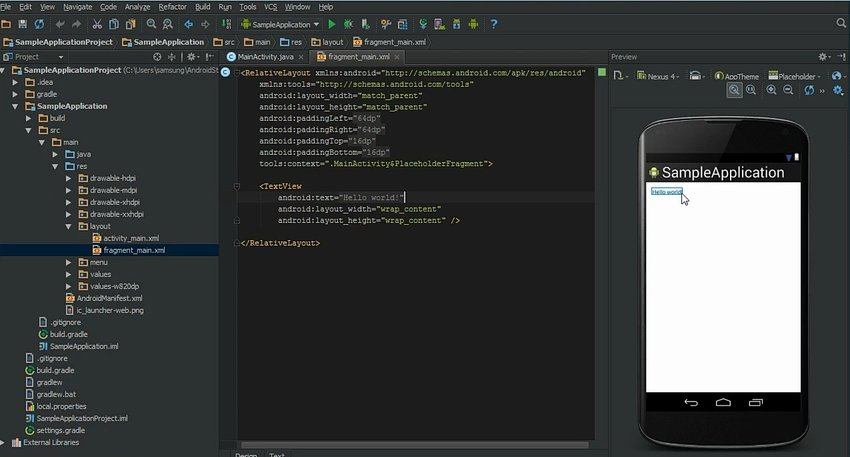
\includegraphics[width=1\linewidth]{images/Android-Studio-user-interface-during-the-development-of-Android-mobile-App-Figure.jpg}\\[1ex]
    \centering
    \caption{Benutzeroberfläche Android Studio\cite{researchgate_android_studio}}
    \label{ABBILDUNG 76}
\end{figure}

Ein entscheidender Vorteil liegt in der Integration aller relevanten Entwicklungsaspekte in einer einzigen
 Umgebung. Dank des eingebauten Build-Systems Gradle lassen sich verschiedene Konfigurationen (z. B. Debug- und Release-Versionen) 
 zentral verwalten, was insbesondere in größeren Entwicklerteams zu einer strukturierten und reproduzierbaren Arbeitsweise beiträgt. 
 Darüber hinaus stellt Android Studio eine visuelle Layout-Ansicht bereit, in der UI(User Interface)-Komponenten per Drag-and-Drop platziert werden können. 
 Änderungen an der Benutzeroberfläche sind sofort sichtbar, ohne dass die App jedes Mal neu kompiliert werden muss.

Der Einsatz von Android Studio wird zudem durch die große Community gestützt, die Anleitungen, Tutorials und Hilfestellungen bietet. 
Damit ist ein schneller Einstieg gewährleistet, selbst wenn Entwickler*innen erst geringe Vorkenntnisse in der nativen Android-Programmierung haben.

Bei der Entwicklung der in dieser Arbeit beschriebenen App wurde hauptsächlich Java als Programmiersprache verwendet. Java ist eine der 
bevorzugten Sprachen für die Android-Entwicklung, da sie von Android nativ unterstützt wird und über eine große Anzahl an Bibliotheken und 
Frameworks verfügt. Durch die weitreichende Unterstützung in Android Studio und die langjährige Etablierung als Standard für Android-Anwendungen 
bietet Java eine zuverlässige und effiziente Grundlage für die Umsetzung komplexer Projekte.

Gleichwohl existieren auch mögliche Einschränkungen. So benötigt Android Studio aufgrund der umfangreichen Funktionalitäten einen 
leistungsfähigen Computer mit ausreichend Arbeitsspeicher; auf schwächeren Systemen kann es zu langen Ladezeiten kommen. Zudem sind 
Entwickler*innen stark an das Google-Ökosystem gebunden, was einerseits für eine gute Integration sorgt, andererseits aber den Handlungsspielraum 
in Bereichen wie Cross-Plattform-Entwicklung begrenzen kann. Wer Android Studio für plattformübergreifende Frameworks (etwa Flutter oder React Native) 
einsetzen möchte, muss zusätzliche Plug-ins einrichten und mit größeren Konfigurationsaufwänden rechnen.

Insgesamt überwiegen die Vorteile von Android Studio, insbesondere in Bezug auf die native Android-Entwicklung. 
Die integrierte Entwicklungsumgebung erleichtert den gesamten Prozess von der ersten Codezeile bis zur Veröffentlichung der 
Anwendung, sodass sie für diese Studienarbeit eine solide Basis für die Umsetzung der Android-App darstellt.
\end{spacing}


\clearpage

\subsection{Eigenschaften und Funktionen}


\begin{spacing}{1.8}  % Adjust line spacing
\fontsize{14pt}{15pt}\selectfont  % Font size and line spacing

Die im Folgenden vorgestellte Android-App demonstriert exemplarisch, wie eine Anwendung zur Erfassung und Anzeige ermittelter Bluetooth-Geräte 
implementiert werden kann. Hierbei stehen insbesondere das Aktivieren von Bluetooth und die Suche nach sichtbaren Geräten im Vordergrund. 
Die Implementierung erfolgt mithilfe verschiedener Klassen und XML(Extensible Markup Language)-Layouts, die im Quellcodeauszug ersichtlich sind.

\subsubsection{Bluetooth-Erkennung und Warnfunktion}

Zentrale Komponenten dieser App sind das Aktivieren und Deaktivieren von Bluetooth, die Suche nach sichtbaren Geräten und das Auslösen von 
Warnhinweisen (z. B. in Form einer Vibration oder einer Dialogmeldung). Die Hauptlogik befindet sich in der MainActivity\cite{lukiano12_lkw_assist}.

\textbf{Aktivieren des Bluetooth-Adapters\cite{lukiano12_lkw_assist}:} Beim Betätigen des bluetoothButton wird geprüft, ob Bluetooth auf dem Gerät vorhanden und aktiviert ist. 
Ist dies nicht der Fall, fordert die Anwendung mittels eines Intent den oder die Nutzende auf, Bluetooth zu aktivieren:

\begin{lstlisting}
    // Methode zum Umschalten von Bluetooth
    private void toggleBluetooth() {
        // Pruefen, ob das Geraet Bluetooth ueberhaupt unterstuetzt
        if (mBluetoothAdapter == null) {
            Toast.makeText(this, "Bluetooth is not supported on this device",
                           Toast.LENGTH_SHORT).show();
            return;
        }
    
        // Ist Bluetooth ausgeschaltet?
        if (!mBluetoothAdapter.isEnabled()) {
            // System-Dialog, der die Nutzer*innen auffordert, Bluetooth zu aktivieren
            Intent enableBtIntent =
                    new Intent(BluetoothAdapter.ACTION_REQUEST_ENABLE);
            enableBluetoothLauncher.launch(enableBtIntent);
        } else {
            // Bluetooth bereits aktiv, daher direkt Discovery starten
            Toast.makeText(this, "Bluetooth is already on", Toast.LENGTH_SHORT).show();
            startBluetoothDiscovery();
        }
    }
    \end{lstlisting}

    \begin{figure}[H]
        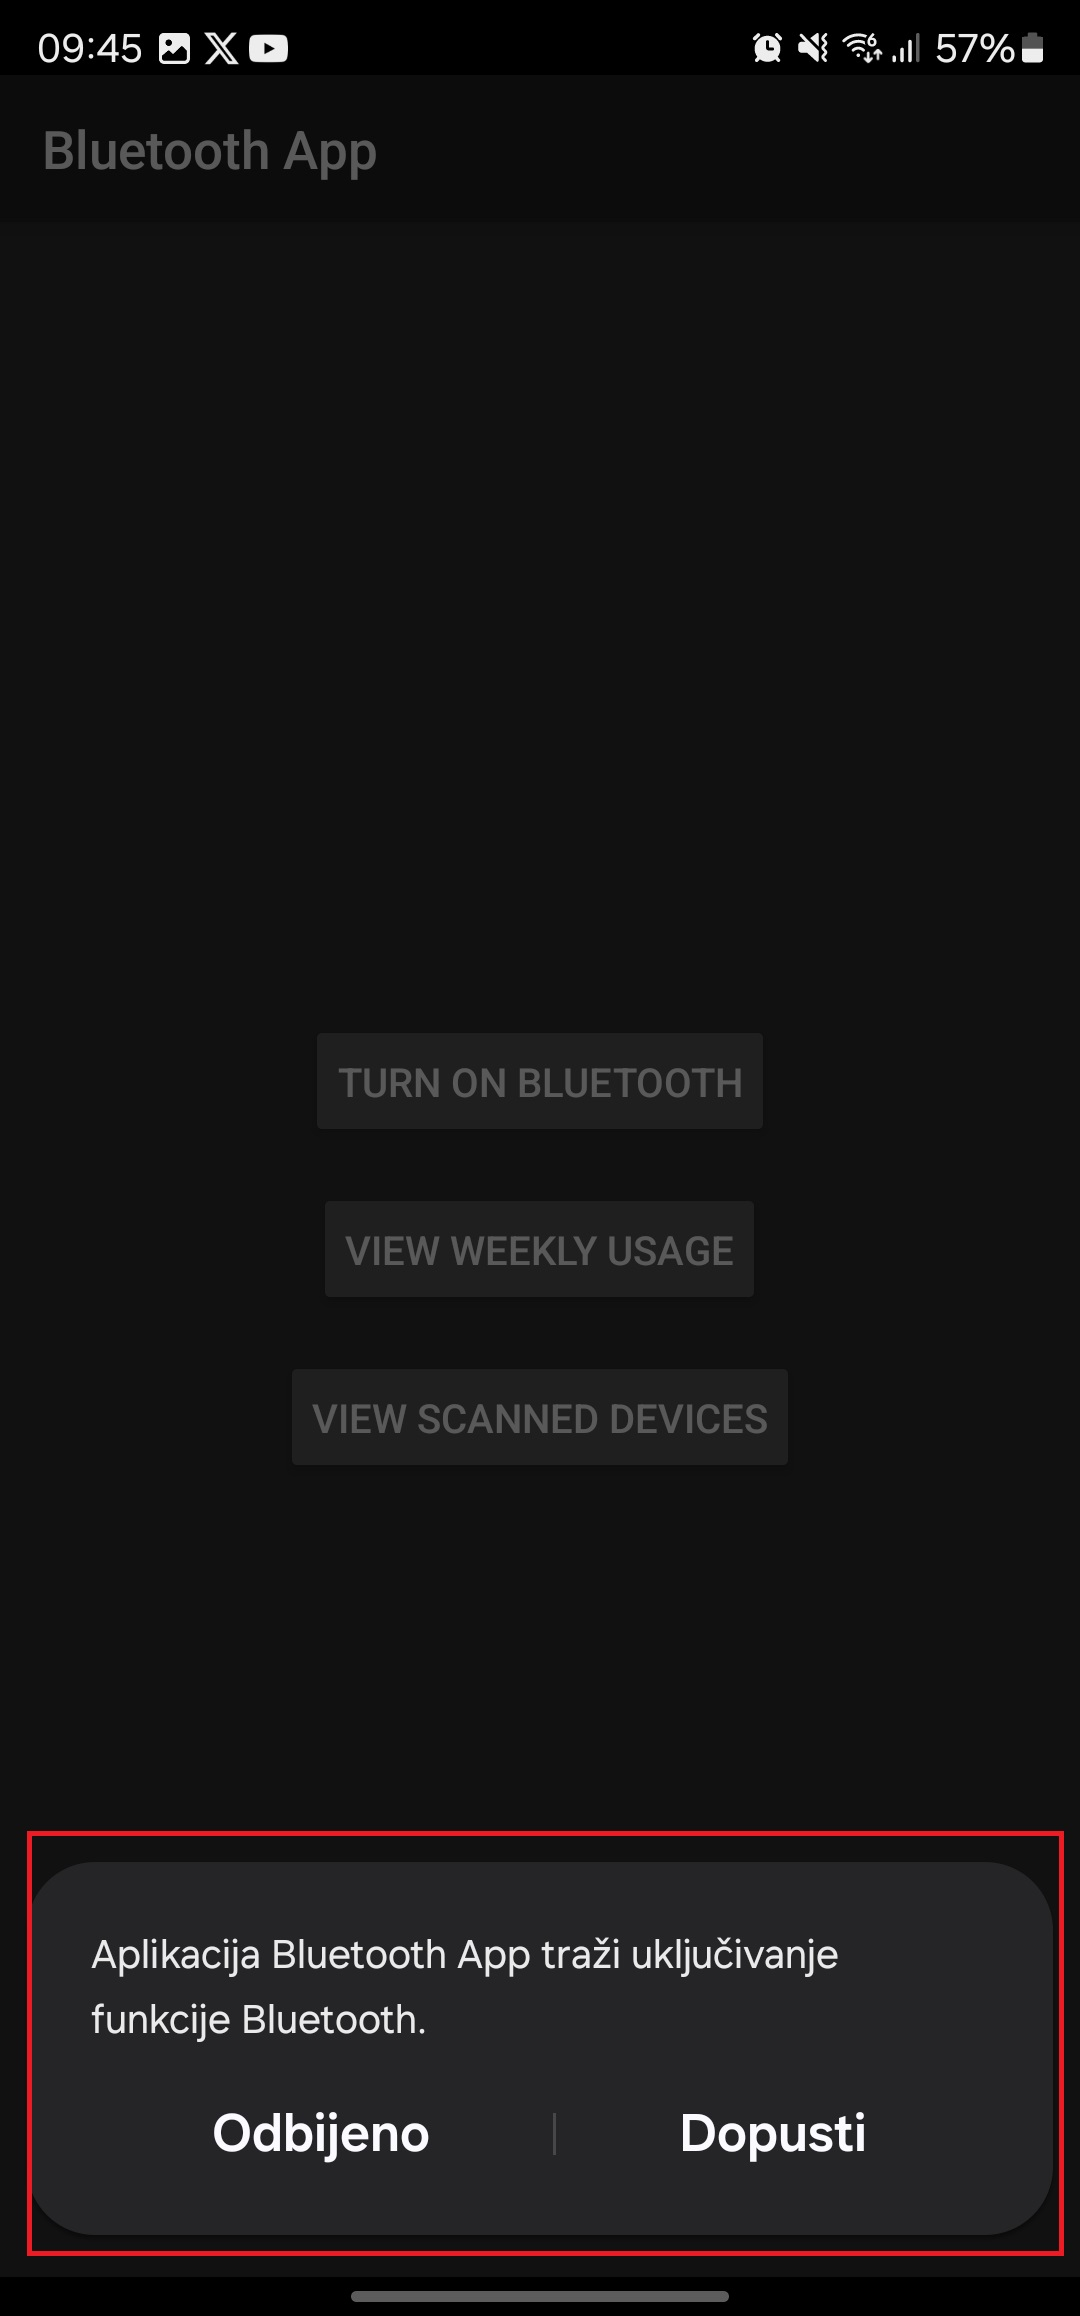
\includegraphics[width=0.5\linewidth]{images/Screenshot_20250113_094518_Settings.jpg}\\[1ex]
        \centering
        \caption{Pop-Up, der den User fragt, Bluetooth zu aktivieren\cite{lukiano12_lkw_assist}}
        \label{ABBILDUNG 76}
    \end{figure}

\textbf{Scanning von Bluetooth-Geräten\cite{lukiano12_lkw_assist}:} Sobald Bluetooth aktiv ist, wird mittels \texttt{startDiscovery()} nach sichtbaren Geräten gesucht. 
Dabei registriert sich die Anwendung im BroadcastReceiver (\texttt{bluetoothReceiver}) für das Ereignis \texttt{BluetoothDevice.ACTION\_FOUND}, um gefundene Geräte abzufangen:

\begin{lstlisting}
    // Methode zum Starten des Bluetooth-Discovery-Vorgangs
    private void startBluetoothDiscovery() {
        // Ab Android 12 (API-Level 31) sind zusaetzliche Berechtigungen noetig
        if (Build.VERSION.SDK_INT >= Build.VERSION_CODES.S) {
            if (ContextCompat.checkSelfPermission(this, Manifest.permission.BLUETOOTH_SCAN)
                    != PackageManager.PERMISSION_GRANTED) {
                ActivityCompat.requestPermissions(this,
                        new String[]{Manifest.permission.BLUETOOTH_SCAN}, 0);
                return;
            }
        }
    
        try {
            // Falls noch ein alter Scan laeuft, abbrechen
            if (mBluetoothAdapter.isDiscovering()) {
                mBluetoothAdapter.cancelDiscovery();
            }
            // Scan nach sichtbaren Bluetooth-Geraeten starten
            mBluetoothAdapter.startDiscovery();
            Toast.makeText(this, "Scanning for Bluetooth devices...",
                           Toast.LENGTH_SHORT).show();
    
            // Nach 12 Sekunden erneut scannen (Wiederholung)
            bluetoothHandler.postDelayed(bluetoothRunnable, 12000);
    
        } catch (SecurityException e) {
            // Fehlerbehandlung bei fehlenden Berechtigungen
            Toast.makeText(this, "Bluetooth permissions are missing", Toast.LENGTH_SHORT).show();
        }
    }
    \end{lstlisting}

    \begin{figure}[H]
        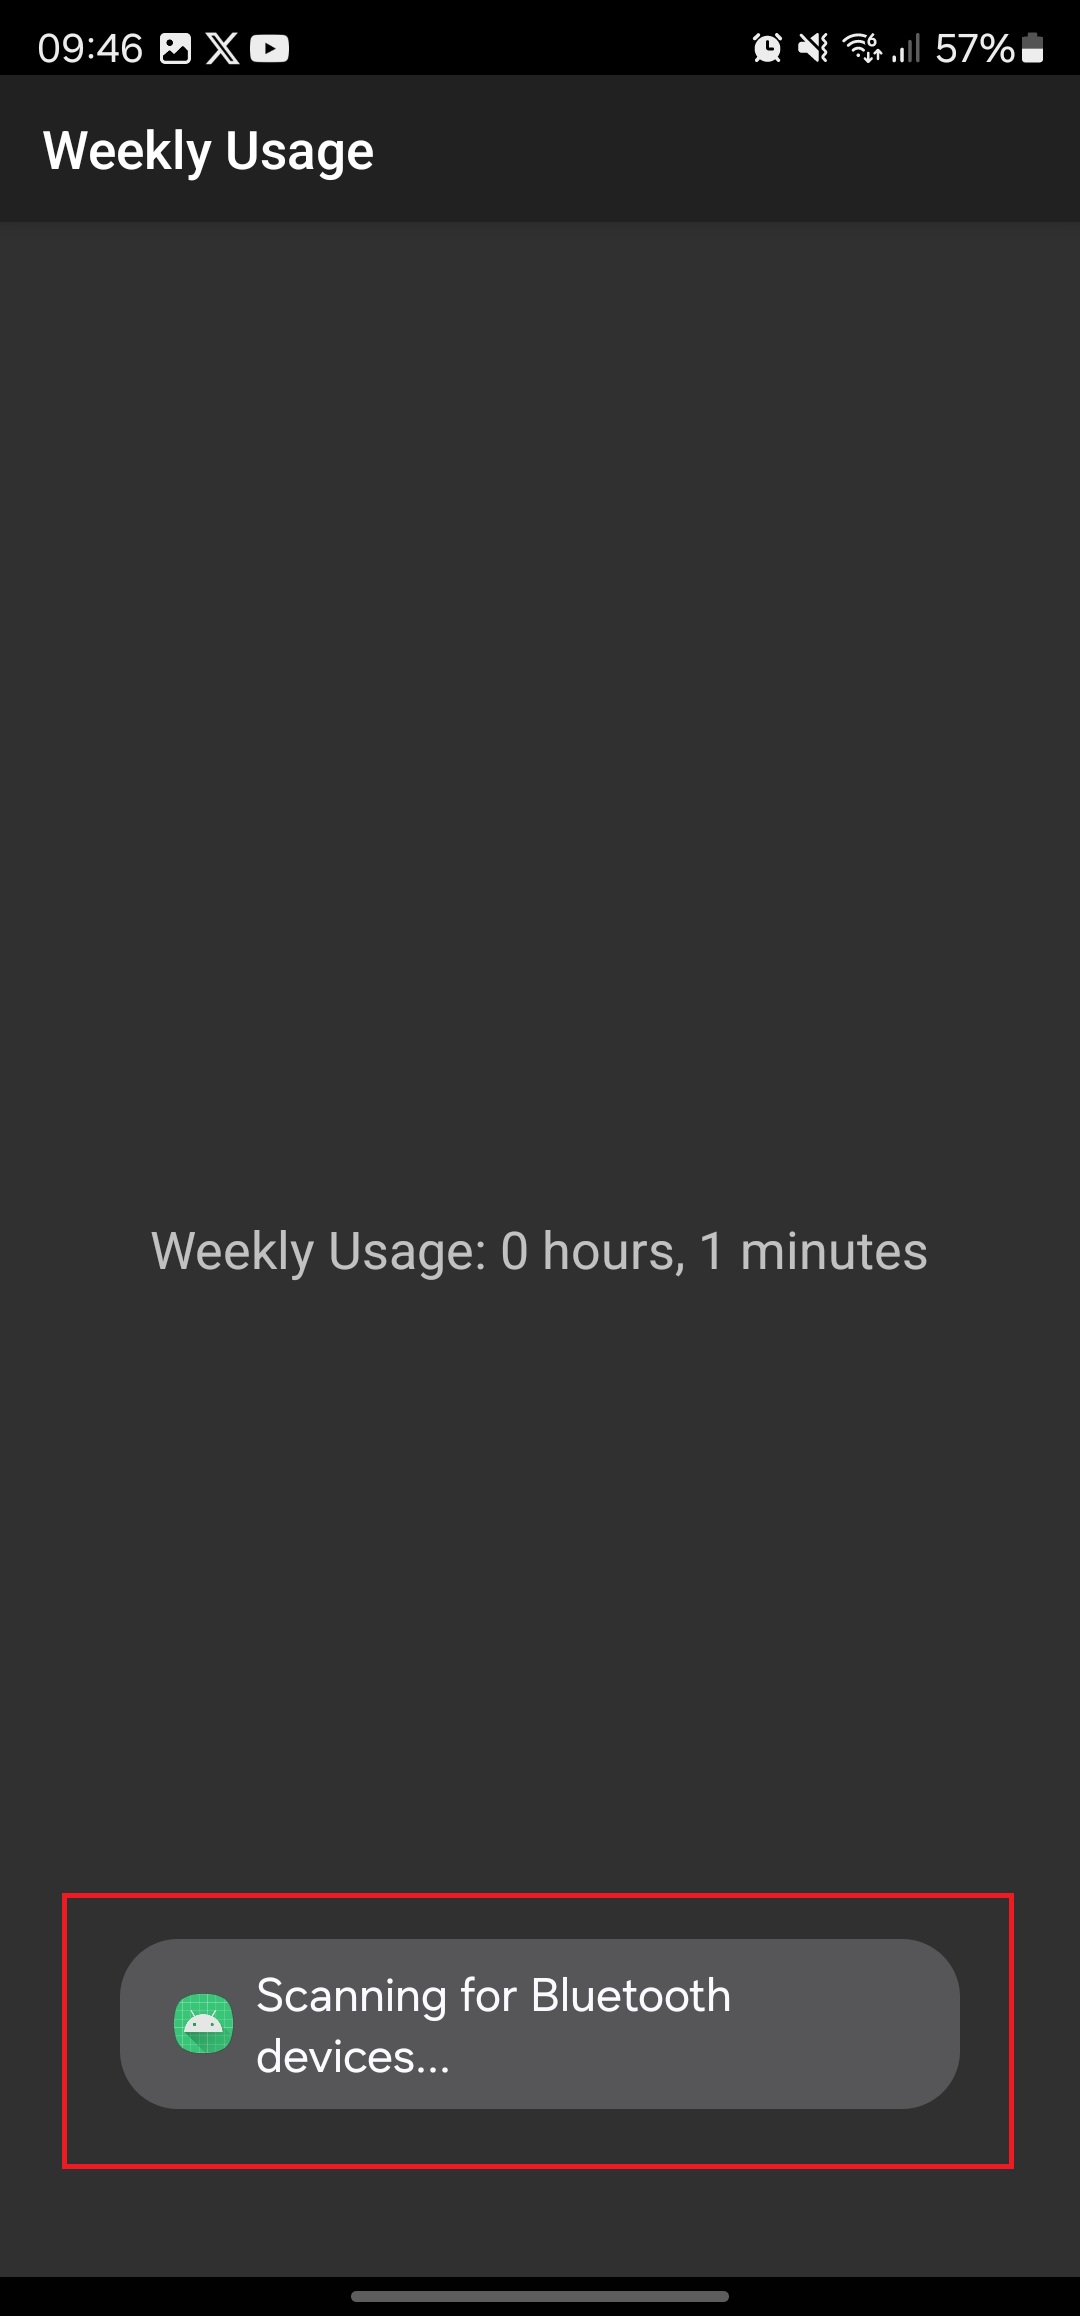
\includegraphics[width=0.5\linewidth]{images/Screenshot_20250113_094628_Bluetooth App.jpg}\\[1ex]
        \centering
        \caption{Beispiel Pop-up Scanning for Bluetooth devices\cite{lukiano12_lkw_assist}}
        \label{ABBILDUNG 76}
    \end{figure}

\textbf{Erkennung neuer Geräte\cite{lukiano12_lkw_assist}:} Für jedes neu erkannte Gerät wird eine Vibration ausgelöst (vibratePhone()), 
und in einem Popup-Fenster (showDeviceDetectedPopup(...)) das gefundene Gerät angezeigt. Zudem wird die Gerätebezeichnung in einer ArrayList (scannedDevicesList) gespeichert:

\begin{lstlisting}
    // BroadcastReceiver, der auf gefundene Bluetooth-Geraete reagiert
    private final BroadcastReceiver bluetoothReceiver = new BroadcastReceiver() {
        @Override
        public void onReceive(Context context, Intent intent) {
            if (BluetoothDevice.ACTION_FOUND.equals(intent.getAction())) {
                // Ein neues Geraet wurde gefunden
                BluetoothDevice device =
                        intent.getParcelableExtra(BluetoothDevice.EXTRA_DEVICE);
    
                if (device != null) {
                    String deviceName = (device.getName() != null)
                                        ? device.getName()
                                        : "Unknown Device";
    
                    // Pruefen, ob dieses Geraet bereits erkannt wurde
                    if (!detectedDevices.contains(deviceName)) {
                        // Neues Geraet -> hinzufuegen und Warnhinweise ausloesen
                        detectedDevices.add(deviceName);
                        scannedDevicesList.add(deviceName);
    
                        vibratePhone();  // Vibration
                        showDeviceDetectedPopup(deviceName);  // Popup-Dialog
                    }
                }
            }
            // ...
        }
    };
    \end{lstlisting}

    \begin{figure}[H]
        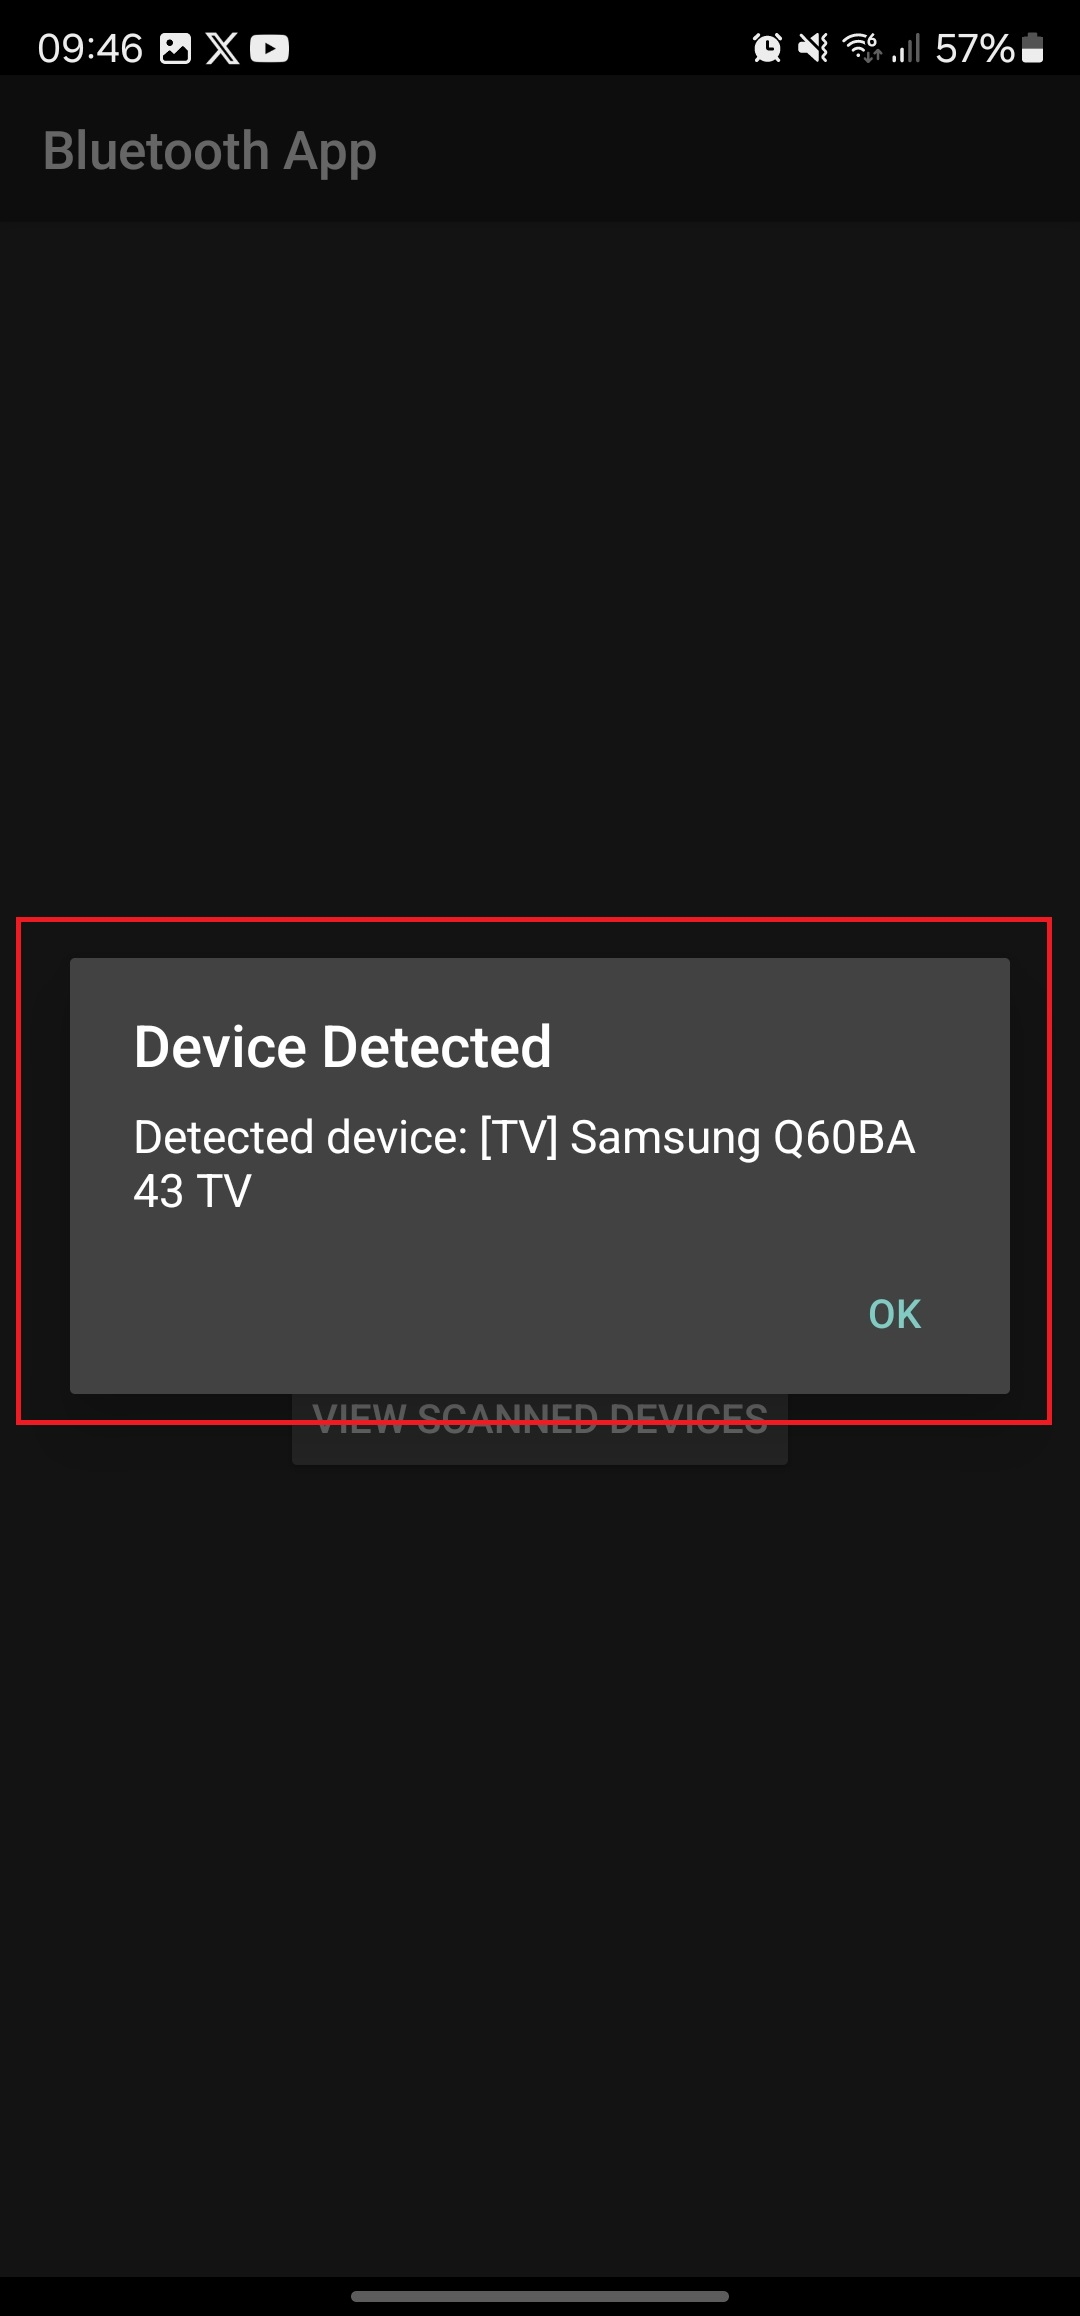
\includegraphics[width=0.5\linewidth]{images/Screenshot_20250113_094600_Bluetooth App.jpg}\\[1ex]
        \centering
        \caption{Pop-Up, der darstellt, welches Bluetooth Gerät erkannt worden ist\cite{lukiano12_lkw_assist}}
        \label{ABBILDUNG 76}
    \end{figure}

   
\textbf{Erneutes Scannen\cite{lukiano12_lkw_assist}:} Nach Ablauf eines festgelegten Zeitintervalls (hier 12 Sekunden) wird das Scannen erneuert (postDelayed(bluetoothRunnable, 12000)), 
solange Bluetooth aktiv bleibt und weitere Geräte in der Nähe sein könnten:

\begin{lstlisting}
    else if (BluetoothAdapter.ACTION_DISCOVERY_FINISHED.equals(action)) {
        // Discovery ist beendet.
        // Nach einer kurzen Wartezeit (1 Sekunde) erneut starten
        bluetoothHandler.postDelayed(bluetoothRunnable, 1000);
    }
    \end{lstlisting}

\textbf{Vibrationswarnung\cite{lukiano12_lkw_assist}:} Zur Warn- oder Hinweisausgabe nutzt die Anwendung die Vibrationsfunktion über das Vibrator-Interface. 
Abhängig von der Android-Version (ab Android 8.0 mit VibrationEffect) werden angepasste Vibrationsschemata realisiert:

\begin{lstlisting}
    // Methode zum Ausloesen einer kurzen Vibration (500ms)
    private void vibratePhone() {
        try {
            if (vibrator != null) {
                if (Build.VERSION.SDK_INT >= Build.VERSION_CODES.O) {
                    // Ab Android 8.0: VibrationEffect nutzbar
                    vibrator.vibrate(VibrationEffect.createOneShot(
                            500, VibrationEffect.DEFAULT_AMPLITUDE));
                } else {
                    // Aeltere Geraete nutzen die ueberladene vibrate(long) Methode
                    vibrator.vibrate(500);
                }
            }
        } catch (SecurityException e) {
            Toast.makeText(this, "Vibration permission is missing", Toast.LENGTH_SHORT).show();
        }
    }
}
// Methode zum Anzeigen eines Dialogfensters bei neuem Geraet
private void showDeviceDetectedPopup(String deviceName) {
    runOnUiThread(() -> {
        AlertDialog.Builder builder = new AlertDialog.Builder(this);
        builder.setTitle("Device Detected");
        builder.setMessage("Detected device: " + deviceName);
        builder.setPositiveButton("OK", (dialog, which) -> dialog.dismiss());
        builder.create().show();
    });
}
    \end{lstlisting}

\subsubsection{Geräteverwaltung und Anzeigefunktionen}
\textbf{ScannedDevicesActivity\cite{lukiano12_lkw_assist}:} Die von der MainActivity übergebene Liste erkannter Geräte (scannedDevicesList) wird in dieser Activity mithilfe eines ListView visualisiert. 
Einfache ArrayAdapter-Elemente dienen zur Anzeige der Gerätenamen. 
Dadurch erhalten Nutzer*innen einen Überblick über alle während der Laufzeit entdeckten Bluetooth-Geräte:

\begin{lstlisting}
    // Zweite Activity zur Anzeige der gefundenen Geraete
    @Override
    protected void onCreate(Bundle savedInstanceState) {
        super.onCreate(savedInstanceState);
        setContentView(R.layout.activity_scanned_devices);
    
        // ListView fuer die Geraetenamen
        ListView scannedDevicesListView = findViewById(R.id.scannedDevicesListView);
    
        // Empfang der Liste erkannter Geraete ueber getIntent()
        ArrayList<String> scannedDevicesList =
                getIntent().getStringArrayListExtra("scannedDevicesList");
    
        // ArrayAdapter fuer einfache Darstellung in der ListView
        ArrayAdapter<String> adapter = new ArrayAdapter<>(
                this, android.R.layout.simple_list_item_1, scannedDevicesList
        );
        scannedDevicesListView.setAdapter(adapter);
    }
    \end{lstlisting}

    \begin{figure}[H]
        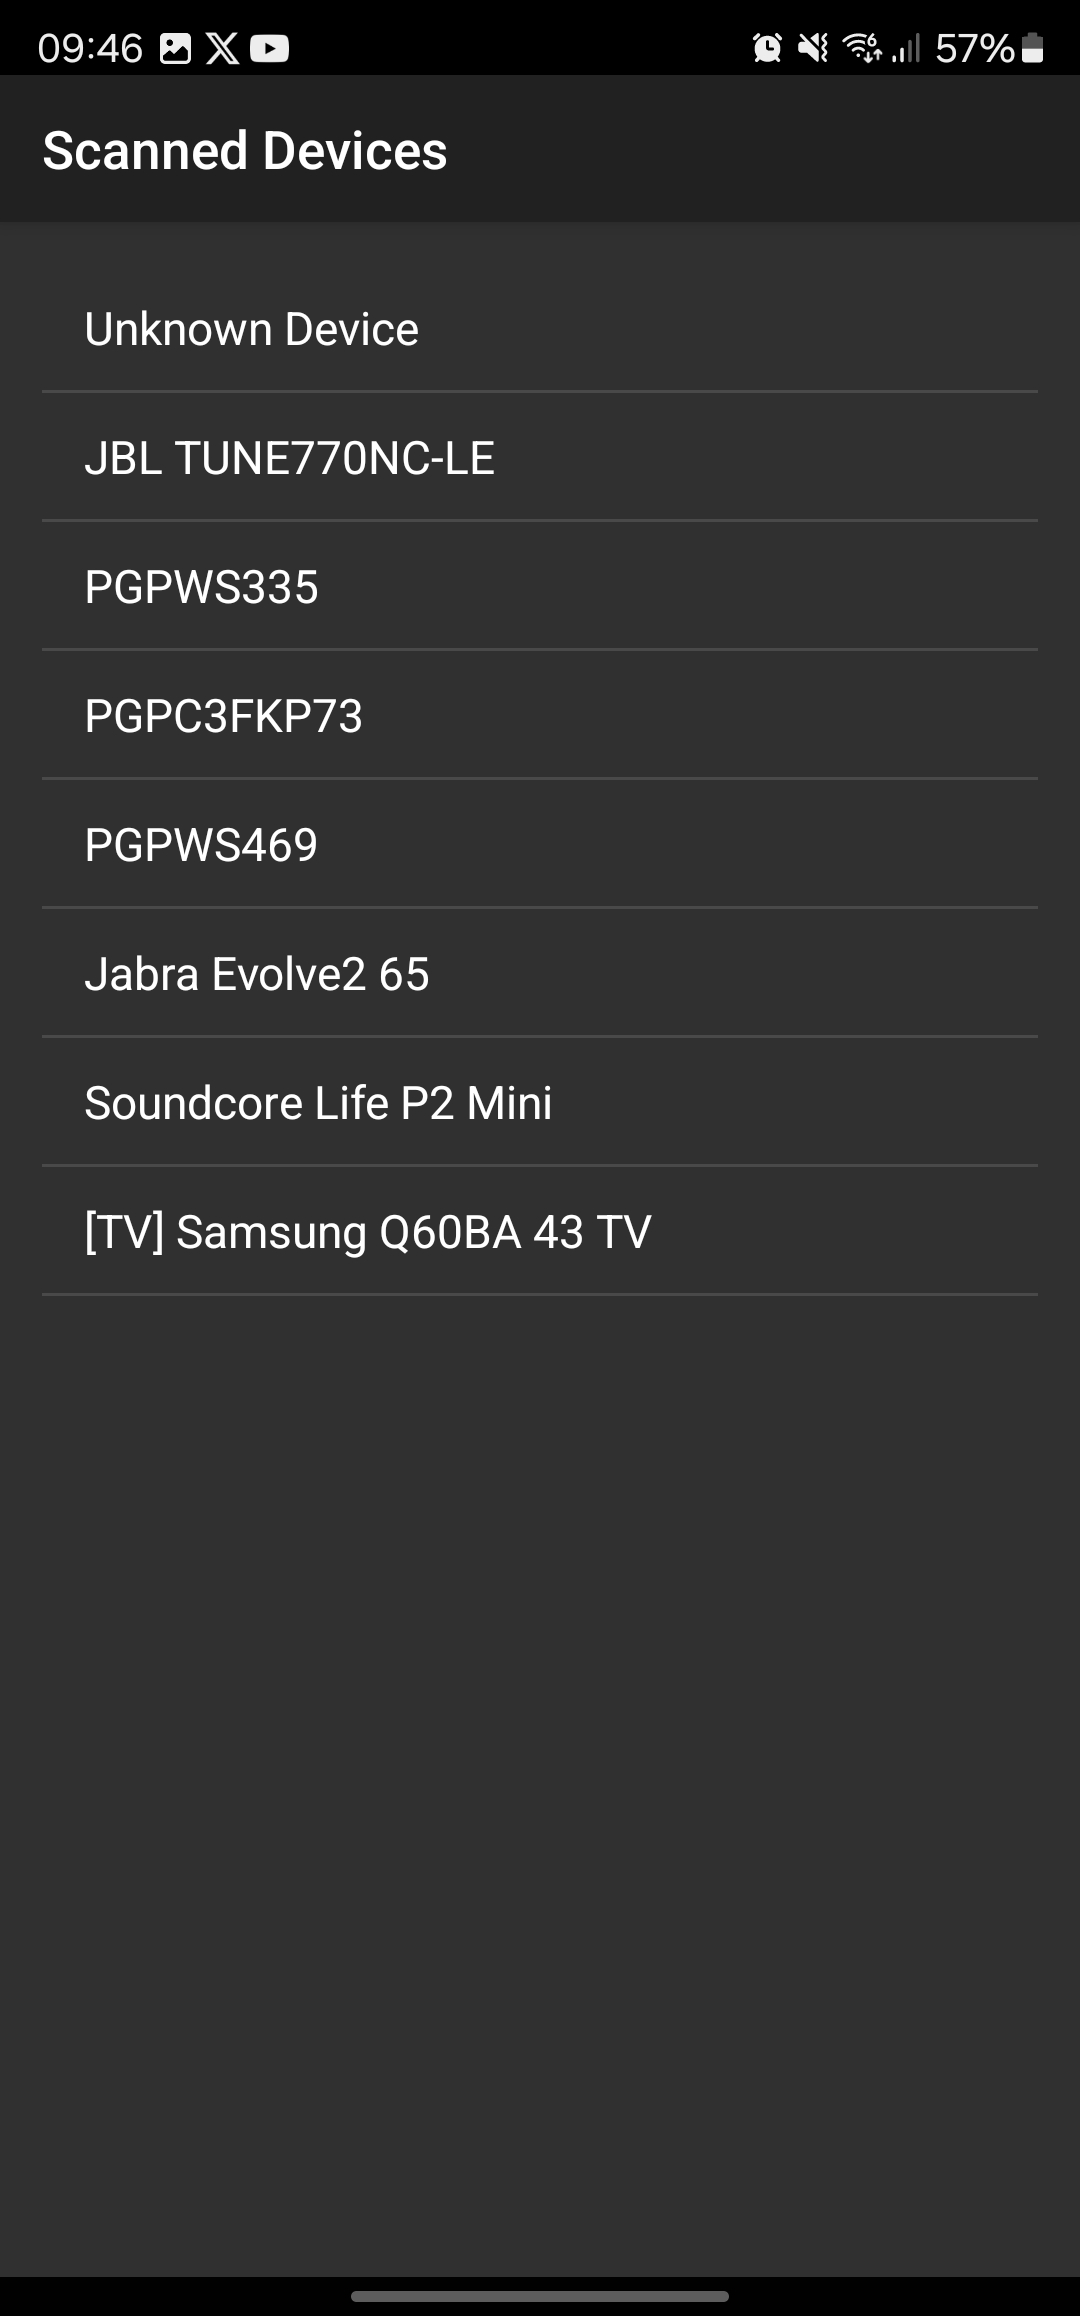
\includegraphics[width=0.5\linewidth]{images/Screenshot_20250113_094607_Bluetooth App.jpg}\\[1ex]
        \centering
        \caption{Liste der erkannent bzw. gescannten Bluetooth-Geräte\cite{lukiano12_lkw_assist}}
        \label{ABBILDUNG 76}
    \end{figure}

\subsubsection{Layout und Benutzeroberfläche}
Die grafische Darstellung der App erfolgt über verschiedene XML-Dateien, die einerseits die Anordnung von Schaltflächen und Textfeldern definieren und andererseits die 
Logik zur Navigation zwischen den Ansichten unterstützen:

\textbf{activity\_main.xml\cite{lukiano12_lkw_assist}:} Enthält drei Schaltflächen für das Ein- oder Ausschalten von Bluetooth, die Anzeige der wöchentlichen Nutzungszeit und die Anzeige der erkannten Geräte.

\textbf{activity\_scanned\_devices.xml\cite{lukiano12_lkw_assist}:} Stellt eine Listenansicht (ListView) bereit, in welcher die erkannten Bluetooth-Geräte angezeigt werden.

Die klare Strukturierung der Layouts ermöglicht einen intuitiven Aufbau der Benutzeroberfläche. Durch den Verzicht auf übermäßig 
komplexe Design-Elemente bleiben sämtliche Hauptfunktionen (Bluetooth-Scan und Geräteliste) leicht zugänglich.

\subsubsection{Berechtigungen und Manifest-Konfiguration}
In der Datei AndroidManifest.xml sind alle nötigen Berechtigungen und Activity-Deklarationen aufgeführt:

\textbf{Bluetooth-Berechtigungen\cite{lukiano12_lkw_assist}:} Die App benötigt verschiedene Berechtigungen, um Bluetooth zu verwenden. Ältere Android-Versionen (bis Android 11) benötigen etwa
 android.permission.BLUETOOTH und android.permission.BLUETOOTH\_ADMIN, während neuere Versionen (ab Android 12, API-Level 31)
  zusätzlich android.permission.BLUETOOTH\_CONNECT und android.permission.BLUETOOTH\_SCAN fordern.

\textbf{Vibrationsberechtigung\cite{lukiano12_lkw_assist}:} Für das Auslösen der Vibration wird die Berechtigung android.permission.VIBRATE definiert, die ab bestimmten Android-Versionen separat eingefordert werden kann.

\textbf{Activities\cite{lukiano12_lkw_assist}:} Sowohl die MainActivity als auch die ScannedDevicesActivity werden 
im Manifest eingetragen, damit das System sie beim App-Start bzw. bei der Navigation zwischen den Bildschirmen korrekt erkennen kann.

\begin{lstlisting}
    % Bluetooth-Berechtigungen fuer die App
<uses-permission android:name="android.permission.BLUETOOTH" />
%  Erlaubt der App, grundlegende Bluetooth-Funktionen zu verwenden 

<uses-permission android:name="android.permission.BLUETOOTH_ADMIN" />
% Ermoeglicht der App, Bluetooth zu verwalten (z. B. Ein-/Ausschalten, Sichtbarkeitssteuerung) 

<uses-permission android:name="android.permission.BLUETOOTH_CONNECT" />
%  Ab Android 12 (API-Level 31) erforderlich: Berechtigung, um Geraete ueber Bluetooth zu verbinden 

<uses-permission android:name="android.permission.BLUETOOTH_SCAN" />
%  Ab Android 12 (API-Level 31) erforderlich: Berechtigung, um nach Bluetooth-Geraeten zu suchen 

<uses-permission android:name="android.permission.VIBRATE" />
%  Ermoeglicht der App, das Geraet durch Vibrationen zu benachrichtigen 

<uses-permission android:name="android.permission.ACCESS_FINE_LOCATION" />
% Ermoeglicht Zugriff auf genaue Standortinformationen; kann fuer BLE-Scanning notwendig sein 

<uses-permission android:name="android.permission.ACCESS_COARSE_LOCATION" />
% Ermoeglicht Zugriff auf ungenaue Standortinformationen; nuetzlich fuer allgemeine Bluetooth-Nutzung 

% Definition der Anwendung und ihrer Activities 
<application
    android:allowBackup="true"
    android:icon="@mipmap/ic_launcher"
    android:label="@string/app_name"
    android:theme="@style/Theme.AppCompat.DayNight">
    % "allowBackup": Ermoeglicht automatische Backups der App-Daten 

    %  Haupt-Activity der App -->
    <activity
        android:name=".MainActivity"
        android:label="@string/app_name"
        android:exported="true">
        % "exported": Legt fest, dass diese Activity von externen Anwendungen gestartet werden kann 
        <intent-filter>
            <action android:name="android.intent.action.MAIN" />
            %  Legt diese Activity als Einstiegspunkt der App fest 
            <category android:name="android.intent.category.LAUNCHER" />
            %  Markiert diese Activity als "Launch-Activity", die beim Starten der App angezeigt wird 
        </intent-filter>
    </activity>

    %  Zusaetzliche Activity zur Anzeige erkannter Geraete 
    <activity
        android:name=".ScannedDevicesActivity"
        android:label="Scanned Devices"
        android:exported="false" />
        %  "exported": Diese Activity kann nur von der eigenen App gestartet werden (nicht von externen Anwendungen) 
</application>

    \end{lstlisting}

    \begin{figure}[H]
        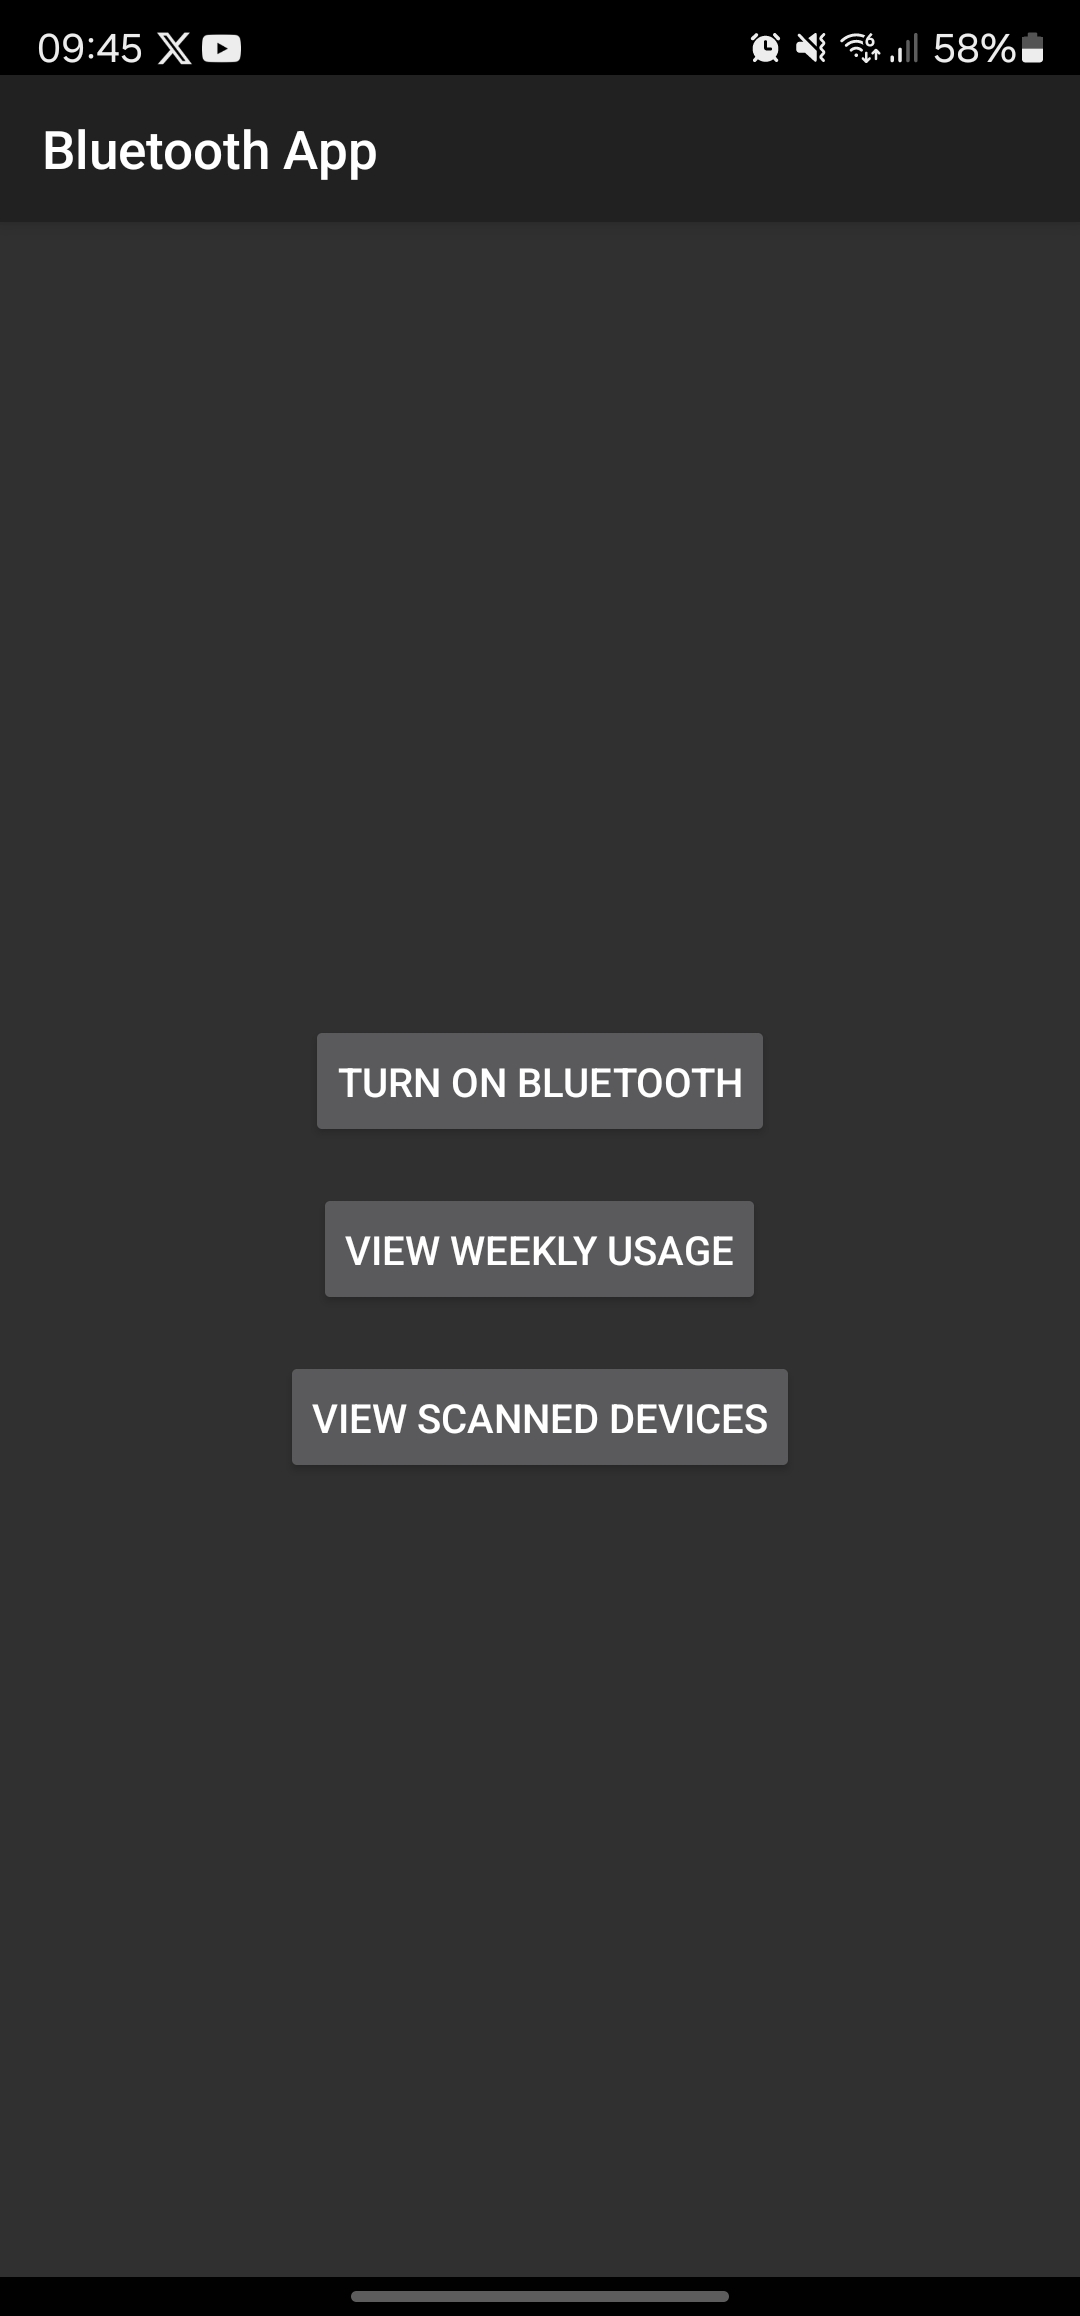
\includegraphics[width=0.5\linewidth]{images/Screenshot_20250113_094506_Bluetooth App.jpg}\\[1ex]
        \centering
        \caption{Aktuelles Aussehen der App mit der derzeitigen Funktionen\cite{lukiano12_lkw_assist}}
        \label{ABBILDUNG 76}
    \end{figure}

In dieser App wird verdeutlicht, wie mithilfe des Bluetooth-Frameworks von Android Geräte in der Umgebung erfasst und entsprechende Warnhinweise an 
die Nutzer*innen ausgegeben werden können. Vom Ein- und Ausschalten von Bluetooth über das Gerätescannen bis hin zur Benutzerinteraktion 
(z. B. Vibration, Pop-up-Dialog) deckt die Anwendung grundlegende Funktionalitäten eines BLE-gestützten Systems ab. 
Die klare Strukturierung in getrennten Activities und XML-Layouts ermöglicht dabei eine einfache Erweiterung und Anpassung der Applikation.
\end{spacing}

\clearpage

\section{Problematik}


\begin{spacing}{1.8}  % Adjust line spacing
\fontsize{14pt}{15pt}\selectfont  % Font size and line spacing

Die Entwicklung der mobilen Anwendung hat bislang große Fortschritte gemacht, insbesondere in Bezug auf die Implementierung der Bluetooth-Scanning-Funktionalität sowie der Benachrichtigungs- und Anzeigeoptionen. Dennoch gibt es eine entscheidende Herausforderung, 
die das Produkt daran hindert, seine vollständige Funktionalität zu erreichen.

Ein zentrales Ziel des Projekts bestand darin, dass die App sowohl als Empfänger
 als auch als Sender arbeiten kann (siehe Kapitel ~\ref{sec:Idee und Konzept}). Bislang ist es jedoch nur möglich, dass die App Bluetooth-Signale 
 empfängt und analysiert. Die angestrebte Funktion, mit der die App konkrete Signale an ein XPLR-Empfängerboard 
 senden könnte, wurde nicht vollständig umgesetzt. Dies ist ein kritischer Aspekt, da die Signalübermittlung erforderlich 
 ist, um den Fahrer eines LKW rechtzeitig vor ungeschützten Verkehrsteilnehmenden, wie Fußgänger*innen oder Fahrradfahrenden, zu warnen.

\subsection{Ursachen des Problems}
\textbf{Fehlende Senderfunktionalität der App:}
Obwohl die App in der Lage ist, verschiedene Bluetooth-Signale zu empfangen, 
gibt es bislang keine Implementierung, mit der die App als Signalquelle (Sender) fungieren kann. 
Dies ist insbesondere für die Kommunikation mit dem XPLR-Empfängerboard von zentraler Bedeutung.

\textbf{Unklare Kompatibilität zwischen Handy und XPLR-Empfängerboard:}
Es wurde versucht, Informationen direkt von der Herstellerfirma des 
XPLR-Boards zu erhalten, um herauszufinden, ob eine direkte Kopplung zwischen einem Smartphone 
und den Empfängerboards technisch möglich ist. Leider konnte bis zum aktuellen Entwicklungsstand 
keine rechtzeitige und konkrete Rückmeldung seitens der Firma eingeholt werden.

Das fehlende Sender-Modul stellt eine erhebliche Einschränkung 
für die angestrebte Anwendung dar. Die Funktion, über Bluetooth gezielte Warnsignale an 
das XPLR-Board zu senden, ist ein wesentlicher Schritt zur Realisierung einer umfassenden und bidirektionalen 
Kommunikationsinfrastruktur. Diese Problematik muss daher in einer Fortsetzung des Projekts prioritär untersucht werden.

\end{spacing}

\clearpage

\section{Aussicht}




\begin{spacing}{1.8}  % Adjust line spacing
\fontsize{14pt}{15pt}\selectfont  % Font size and line spacing

Die vorliegende Studienarbeit hat wesentliche Grundlagen für die Entwicklung einer mobilen 
Anwendung zur Verbesserung der Verkehrssicherheit geschaffen. Dennoch bleibt Potenzial für weitere Arbeiten und Verbesserungen, die die
 Funktionalität und den Nutzen der App erweitern können.

Ein wichtiger Aspekt für zukünftige Entwicklungen ist die Optimierung der Benutzeroberfläche. 
Die App sollte benutzerfreundlich gestaltet werden, sodass alle Altersgruppen sie intuitiv nutzen können. 
Zudem könnten weitere Funktionen wie ein Dark Mode und barrierefreie Optionen integriert werden, um den Komfort und die Zugänglichkeit zu erhöhen.

Ein vielversprechender Ansatz für eine Erweiterung ist die Integration von Kartenmaterial. Mit der Darstellung
 potenzieller Gefahrenzonen oder der Möglichkeit, sicherere Routen für Fußgänger*innen und Fahrradfahrende anzuzeigen,
  könnte die App einen zusätzlichen Beitrag zur Verkehrssicherheit leisten. Auch die Einbindung von Echtzeitdaten aus öffentlichen 
  Quellen, beispielsweise zu Baustellen oder Verkehrsunfällen, würde die Relevanz der App erhöhen.

Darüber hinaus könnte ein Notfallmanagement integriert werden, das automatisierte Notrufoptionen und die Möglichkeit 
bietet, im Ernstfall hinterlegte Kontakte zu benachrichtigen. Ergänzt durch eine erste Hilfe-Anleitung könnte die App so auch in 
kritischen Situationen unterstützend wirken.

Ein zentraler technischer Schwerpunkt sollte jedoch weiterhin die Entwicklung der Senderfunktion bleiben. Die App
 sollte in der Lage sein, nicht nur Bluetooth-Signale zu empfangen, sondern auch gezielt Warnsignale an ein XPLR-Empfängerboard
  oder ähnliche Geräte zu senden. Dies erfordert sowohl eine technische Klärung der Kompatibilität als auch die Entwicklung eines
   Kommunikationsprotokolls. Diese Funktion ist entscheidend, um die App vollständig bidirektional zu gestalten und so ihre Einsatzmöglichkeiten zu maximieren.

Abschließend wäre eine plattformübergreifende Entwicklung, insbesondere für iOS, ein weiterer wichtiger Schritt, 
um eine größere Nutzerbasis anzusprechen. Mit der Übersetzung in mehrere Sprachen und der Einbindung neuer Technologien wie
 Machine Learning könnten darüber hinaus zukünftige Versionen der App international und technologisch führend sein.

Diese Ausblick zeigt auf, dass die App ein solides Fundament für weitere Entwicklungen bietet und das Potenzial 
hat, einen erheblichen Beitrag zur Erhöhung der Verkehrssicherheit zu leisten. Damit schließt diese Arbeit mit einem positiven 
Blick in die Zukunft und einer klaren Zielrichtung für die Weiterführung des Projekts.


\end{spacing}

\clearpage
%---------------------------------------------------------
% Bibliografie
%---------------------------------------------------------
\begingroup
\renewcommand{\bibfont}{\fontsize{13pt}{12pt}\selectfont}  
\sloppy
\nocite{*}
\printbibliography
\endgroup

\end{document}
